\documentclass{article}
\usepackage[utf8]{inputenc}
\usepackage{graphicx} % images and graphics
\usepackage{amsmath,amssymb,amsfonts,amsthm,mathtools} % Math fonts and equations
\usepackage{latexsym} % Math library
\usepackage{array} % Table library
\usepackage{float} % Force image positions using [H]
\usepackage{siunitx,booktabs,cancel,caption,colortbl,csquotes,helvet,mathpazo,listings,xcolor} % SI units within equations along with formatting packages
\usepackage{multirow,multicol} % Multiple columns and rows
\usepackage{tikz-cd,pgfplots} % Tikz Images and custom figures
\usepackage{physics} % Physics variables and better math notation
\usepackage[margin=1in]{geometry} % Fix margins
\pgfplotsset{compat=1.16} % Version 1.16
\usepackage{mleftright} % Math delimiters for better parenthesis
\usepackage{dirtytalk} % Quotation marks using \say
\usepackage{relsize} % Bigger math
\usepackage[english]{babel} % Theorum
\usepackage{hyperref} % Clickable Links

% THM settings
\newtheorem{theorem}{Theorem}[section]
\newtheorem{corollary}{Corollary}[theorem]
\newtheorem{lemma}[theorem]{Lemma}

\newcommand{\n}{\leavevmode \newline} % One newline without indentation
\newcommand{\nn}{\leavevmode \newline \newline} % Two newlines without indentation
\newcommand{\R}{\mathbb{R}} % Math R
\newcommand{\limxyto}[2]{\lim_{(x,y)\to(#1,#2)}} % Function for limits of 2 variables
\newcommand{\xy}{$(x,y)\,$} % Macro for (x,y)
\newcommand{\fxy}{$f(x,y)\,$} % Macro for f(x,y)
\newcommand{\as}{\text{ as }} % Macro for "as" inside math environment
\newcommand{\Du}{D_{\underline{u}}\,} % Macro for Directional derivative
\newcommand{\first}{$1^{\text{st}}\,$} % 1st
\newcommand{\second}{$2^{\text{nd}}\,$} % 2nd
\newcommand{\third}{$3^{\text{rd}}\,$} % 3rd

\numberwithin{equation}{subsection} % Equation labels include subsection and section


% This document was created by Sharwin Patil and is available on github at [Link]. 
% If you have any questions or feedback, feel free to contact me via my email: sharwin24@gmail.com

\begin{document}
\title{

\includegraphics[width=3.5in]{logo}\\
MATH20060\\
Calculus of Several Variables}
\author{Sharwin Patil\\ sharwin24@gmail.com}
\date{September - December, 2019}
\maketitle

\section*{Introduction}
These notes are for the course MATH20060, taken at the University College Dublin(UCD), during the months of September to December. The title of the course is Calculus of Several Variables, colloquially known as Calculus 3, or Multi-variable Calculus. These notes have been rewritten in \LaTeX\, from my own hand-written notes. If you have any questions or feedback, feel free to contact me via my email.

\tableofcontents

\section{Limits with Several Variables}
Recall that in 1 variable calculus, we can check either the right or left hand limit. This concept remains the same for limits of several variables in the sense that every path to the point \xy, should approach the same value. However with functions of several variables, there are infinite paths that can be taken to approach a point \xy.

\begin{figure}[H]
    \centering
    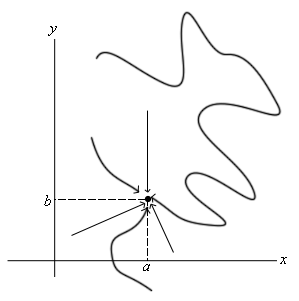
\includegraphics[width=2in]{multiplePaths.png}
    %\caption{Caption}
    %\label{fig:my_label}
\end{figure}
\n
We can use the same concept from single variable calculus to find the limit. A function is continuous at the point (a,b) if

\begin{equation}
    \limxyto{a}{b}f(x,y)=f(a,b)
\end{equation}
\n
Plugging in the point into the function, \fxy, will return the value of the limit. You just need to be careful for division by zero, square roots of negative numbers, logarithms of zero or negative numbers, etc. Additionally, if two different paths approach different values for the limit, it can be concluded that the limit does not exist (DNE).
\nn
Examples:
\nn
\noindent 1. 
\begin{equation}
    \begin{split}
        \limxyto{3}{-4}(x^2+y^2)\\
        \lim_{x\to3}x^2+\lim_{y\to-4}y^2=25
    \end{split}
\end{equation}

\noindent 2.
\begin{equation}
    \begin{split}
        \limxyto{3}{-4}\sqrt{x^2+y^2}\\
        \limxyto{3}{-4}\sqrt{x^2+y^2}=\sqrt{25}=5
    \end{split}
\end{equation}

\noindent 3.
\begin{equation}
    \begin{split}
        \limxyto{0}{1}\frac{x-xy+3}{x^2y+5xy-y^3}\\
        =\frac{0-(0)(1)+3}{(0)^2(1)+5(0)(1)-(1)^3}=-3
    \end{split}
\end{equation}

\noindent 4. Show that the function $f(x,y)=\frac{x^2y}{x^2+y^2}$ has limit 0 at (0,0). $|f(x,y)-\ell|$ becomes arbitrarily small as $(x,y)\rightarrow(0,0)$.

\begin{equation}
    \begin{split}
        |f(x,y)-\ell|=|f(x,y)-0|=\left|\frac{x^2y}{x^2+y^2}\right|=\overbracket{\frac{x^2}{x^2+y^2}}^{\leq 1}\cdot|y|\leq|y|\rightarrow 0\as (x,y)\rightarrow(0,0)
    \end{split}
\end{equation}

So $f(x,y)\rightarrow 0$ as $(x,y)\rightarrow(0,0)$.

\noindent 5.
\begin{equation}
    \begin{split}
        f(x,y)=\frac{x^2y-y^3}{x^2+y^2}
    \end{split}
\end{equation}

Show that the function \fxy has a limit at (0,0). If $f$ has a limit at (0,0) then it must have this limit along any path approaching (0,0).
\nn
On the x-axis we have $f(x,0)=\frac{0}{x^2}=0$. The limit of $f$ (if it exists) must be zero. The function can be rewritten as

\begin{equation}
    \begin{split}
        f(x,y)&=g(x,y)-h(x,y)\\
        g(x,y)&=\frac{x^2y}{x^2+y^2}\\
        h(x,y)&=\frac{y^3}{x^2+y^2}\\
        g(x,y)&\rightarrow 0 \as (x,y)\rightarrow 0\\
        |h(x,y)-0|&=\left|\frac{y^3}{x^2+y^2}\right|=\overbracket{\frac{y^2}{x^2+y^2}}^{\leq 1}\cdot|y|\leq|y|\rightarrow0\as(x,y)\rightarrow(0,0)\\
        f(x,y)&=g(x,y)-h(x,y)\rightarrow 0-0=0 \as (x,y)\rightarrow (0,0)
    \end{split}
\end{equation}

\subsection{Two Path Test}
If \fxy has different limits along 2 different paths approaching \xy then the limit DNE.
\nn
\noindent 1.
\begin{equation}
    f(x,y)=\frac{xy}{x^2+y^2}
\end{equation}
\n
Show that the function's limit does not exist at (0,0). For the limit of $f$ to exist at (0,0), the limit along every curve to (0,0) must exist, and all limits must be equal.
\nn
Along the x-axis, $(x,0)$, we get $f(x,0)=\frac{x\cdot0}{x^2+0}=0$.
\nn
Along the y-axis, $(0,y)$, we get $f(0,y)=\frac{0\cdot y}{0+y^2}=0$.
\nn
Along the line $y=x$, we get $f(x,x)=\frac{x^2}{2x^2}=\frac{1}{2}\neq0$. $\therefore$ the limit of \fxy at (0,0) DNE.
\nn
\noindent 2.
\begin{equation}
    f(x,y)=\frac{2x^2y}{x^4+y^2}
\end{equation}
\n
Does the function \fxy have a limit at (0,0)?
\nn
Along a line, $y=mx$, we get:
\begin{equation}
    f(x,mx)=\frac{2mx^3}{x^4+m^2x^2}=\frac{2mx}{x^2+m^2}\rightarrow0 \as x\rightarrow 0
\end{equation}
\n
Along the curve, $y=kx^2$, we get:
\begin{equation}
    f(x,kx^2)=\frac{2kx^4}{x^4+k^2x^4}=\frac{2k}{1+k^2}\rightarrow\frac{2k}{1+k^2}
\end{equation}
\n
This limit varies depending on $k$, $\therefore$ the limit DNE by the two-path test.
\section{Domains of Multi-Variable Functions}
$D$ is a subset of $\R^2$. A function \fxy assigns each pair \xy in $D$ a value $z=f(x,y)\in\R$. The domain, $D$, is all pairs \xy allowable as input in \fxy. The set of all outputs, \fxy, is the range. $D$ is usually represented graphically with the form:

\begin{equation}
    D=\{(x,y): x,y\}
\end{equation}
\n
With conditional statements in the space for $x$ and $y$ which keep the function \fxy true.
\nn
\noindent 1.
\begin{equation}
    \begin{split}
        f(x,y)&=\sqrt{xy}\\
        D&=\{(x,y):xy\geq0\}
    \end{split}
\end{equation}

\noindent 2.
\begin{equation}
    \begin{split}
        f(x,y)&=\frac{x}{x^2-y^2}\\
        D&=\{(x,y):y>x,y<-x,y\geq0\}
    \end{split}
\end{equation}

\noindent 3.
\begin{equation}
    \begin{split}
        f(x,y,z)&=\frac{1}{x^2+e^{yz}}\\
        D&=\{(x,y,z):\R^3\}
    \end{split}
\end{equation}

\noindent 4.
\begin{equation}
    \begin{split}
        f(x,y)&=\ln(1-\frac{x^2}{y})\\
        D&=\{(x,y):\frac{x^2}{y}>1,y\neq0\}
    \end{split}
\end{equation}

\noindent 5.
\begin{equation}
    \begin{split}
        f(x,y)&=\frac{1}{\sqrt{x^2+y^2-9}}\\
        D&=\{(x,y):||(x,y)||>3\}
    \end{split}
\end{equation}

\noindent 6.
\begin{equation}
    \begin{split}
        f(x,y)&=\frac{1}{\sqrt{x^2+2y^2}-y}\\
        D&=\{(x,y):x>0\,\&\,y>0,\sqrt{x^2+2y^2}>y\}
    \end{split}
\end{equation}
\n
The domain can be split into $\partial D$, the outer domain, and $D^{\circ}$, the inner domain. The two domains create the full domain $\overline{D}$. Depending on the nature of the domain, the domain can be determined to be open or closed.
\nn
\noindent 7.
\begin{equation}
    \begin{split}
        D&=\{(x,y):x\geq0,y>0\}\\
        \partial D&=\{(x,y):x=0\}\\
        D^{\circ}&=\{(x,y):x>0,y>0\}\\
        \overline{D}&=\{(x,y):x\geq0,y>0\}\\
        D&\text{ is open}
    \end{split}
\end{equation}

\noindent 8.
\begin{equation}
    \begin{split}
        D&=\{(x,y):x+y=1\}\\
        \partial D&=\{(x,y):x+y=1\}\\
        D^{\circ}&=\{(x,y):x+y=1\}\\
        \overline{D}&=\{(x,y):x+y=1\}\\
        D&\text{ is closed}
    \end{split}
\end{equation}

\noindent 9.
\begin{equation}
    \begin{split}
        D&=\{(x,y):0\leq x\leq 1\}\\
        \partial D&=\{(x,y):x=0,x=1\}\\
        D^{\circ}&=\{(x,y):0<x<1\}\\
        \overline{D}&=\{(x,y):0\leq x\leq 1\}\\
        D&\text{ is closed}
    \end{split}
\end{equation}

\noindent 10.
\begin{equation}
    \begin{split}
        D&=\{(x,y):x^2+y^2<1,y<0\}\\
        \partial D&=\{(x,y):\,\}\\
        D^{\circ}&=\{(x,y):x^2+y^2<1,y<0\}\\
        \overline{D}&=\{(x,y):x^2+y^2<1,y<0\}\\
        D&\text{ is open}
    \end{split}
\end{equation}
\section{Level Curves}
Graphs of functions with the form $z=f(x,y)$ are called level curves, and level surfaces for the form $F(x,y,z)=c$. The function $z=f(x,y)$ has exactly one $z$ value for \xy in the domain of \fxy, and has no value for \xy outside the domain of \fxy. The graph of the function $z=f(x,y)$ must pass the vertical line test.

\begin{equation}
    \begin{split}
        f(x,y)&=-x^2-2y^2\\
        c&=-x^2-2y^2\\
        1&=\frac{x^2}{-c}+\frac{2y^2}{-c}
    \end{split}
\end{equation}
\n
The level curves for the function \fxy can be graphed for $c=-1,-2,-3,\cdots,-10$.

\begin{figure}[H]
    \centering
    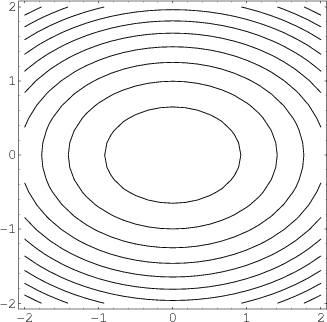
\includegraphics[width=2in]{levelCurves.png}
    %\caption{Caption}
    %\label{fig:my_label}
\end{figure}
\n
A level curve $f(x,y)=c$ can be thought of as a horizontal slice of the graph at height $z=c$. This slice is the intersection of the plane $z=c$ and the function \fxy.
\section{Partial Differentiation}
Recall one-variable differentiation, $f:\R\rightarrow\R$. Include the graphic from the notes.
\nn
Let $f:\R^2\rightarrow\R$. Given $(x_0,y_0)$, the vertical plane $y=y_0$ cuts the surface $z=f(x,y)$ in the curve $z=f(x,y_0)$ (cross section of the graph). The partial derivative $\pdv{f}{x}$ of $f$ with respect to $x$ at $(x_0,y_0)$ is the (ordinary) derivative of the function $x\rightarrow f(x,y_0)$ at $x=x_0$. Geometrically, $\pdv{f}{x}(x_0,y_0)$ is the slope of the line tangent to the trace of the graph of $f$ in the plane $y=y_0$. Similarly, $\pdv{f}{y}(x_0,y_0)$ is the slope of the line tangent to the trace of the graph of $f$ in the plane $x=x_0$.
\nn
The Partial Derivative of \fxy with respect to $x$ at $(x_0,y_0)$ is the number

\begin{equation}
    \begin{split}
        \pdv{f}{x}(x_0,y_0)=\lim_{h\to0}\frac{f(x_0+h,y_0)-f(x_0,y_0)}{h}\\
        \text{Provided that the limit exists}
    \end{split}
\end{equation}
\n
Similarly, the Partial Derivative of \fxy with respect to $y$ at $(x_0,y_0)$ is the number

\begin{equation}
    \begin{split}
        \pdv{f}{y}(x_0,y_0)=\lim_{h\to0}\frac{f(x_0,y_0+h)-f(x_0,y_0)}{h}\\
        \text{Provided that the limit exists}
    \end{split}
\end{equation}
\n
The notation $f_x$ and $f_y$ is often used for $\pdv{f}{x}$ and $\pdv{f}{y}$, respectively.
\nn
Calculation of $f_x$ involves treating $y$ as a constant and then differentiating with respect to $x$. This can usually be done with standard rules of differentiating.

\begin{equation}
    \begin{split}
        f(x,y)&=x^2y\\
        f_x&=2xy\\
        f_y&=x^2
    \end{split}
\end{equation}

\noindent 1.
\begin{equation}
    \begin{split}
        f(x,y)&=x^2y^3+e^x\ln(y)\\
        f_x&=2xy^3+e^x\ln(y)\\
        f_y&=3x^2y^2+\frac{e^x}{y}\\
        f_x(4,1)&=8\\
        f_y(4,1)&=48+e^4
    \end{split}
\end{equation}

\noindent 2.
\begin{equation}
    \begin{split}
        f(x,y)&=\sqrt{9-x^2-y^2}\\
        f_x&=\frac{-x}{\sqrt{9-x^2-y^2}}\\
        f_y&=\frac{-y}{\sqrt{9-x^2-y^2}}\\
        f_x(1,2)&=-\frac{1}{2}\\
        f_y(1,2)&=-1
    \end{split}
\end{equation}

\noindent 3.
\begin{equation}
    f(x,y)=\left\{
    \begin{array}{ll}
        x^2+y^2+z^2=9\\
        z\geq0
    \end{array}
    \right.
\end{equation}
\n
If we're on the surface at (1,2,2), then the slope in the x-direction is $-\frac{1}{2}$, and in the y-direction is $-1$.
\nn
If \fxy is a differentiable function of one variable, show that the function $g(x,y)=f(\frac{x}{y})$ satisfies the \say{partial differential equation} $x\pdv{g}{x}+y\pdv{g}{y}=0$. By the chain rule:

\begin{equation}
    \begin{split}
        g_x&=f'\left(\frac{x}{y}\right)\left(\frac{1}{y}\right)\\
        g_y&=f'\left(\frac{x}{y}\right)\left(-\frac{x}{y^2}\right)\\
        xg_x+yg_y&=f'\left(\frac{x}{y}\right)\left(\frac{x}{y}\right)-f'\left(\frac{x}{y}\right)\left(\frac{x}{y}\right)
    \end{split}
\end{equation}
\n
Partial derivatives are define similarly for functions of more than two variables. In this case, we treat all but one of the variables as constant.

\begin{equation}
    \begin{split}
        f(x,y,z)&=\sqrt{x}e^\frac{y}{z}\\
        f_x&=\frac{e^\frac{y}{z}}{2\sqrt{x}}\\
        f_y&=\frac{\sqrt{x}}{z}e^\frac{y}{z}\\
        f_z&=\sqrt{x}\cdot e^\frac{y}{z}\left(-\frac{y}{z^2}\right)
    \end{split}
\end{equation}

\subsection{Higher Order Partial Derivatives}
Let $f:\R^2\to\R$, then $f_x$ and $f_y$ are also functions from $\R^2\to\R$, so we can consider partial derivatives of them:

\begin{equation}
    \begin{split}
        \pdv[2]{f}{x}&=\pdv{x}(\pdv{f}{x}), \qquad f_{xx}=(f_x)_x\\
        \pdv[2]{f}{y}&=\pdv{y}(\pdv{f}{y}), \qquad f_{yy}=(f_y)_y\\
        \pdv{f}{x}{y}&=\pdv{x}(\pdv{f}{y}), \qquad f_{yx}=(f_y)_x\\
        \pdv{f}{y}{x}&=\pdv{y}(\pdv{f}{x}), \qquad f_{xy}=(f_x)_y
    \end{split}
\end{equation}
\n
$f_{xy}$ and $f_{yx}$ are called mixed partial derivatives and $f_{xx}$ and $f_{yy}$ are called pure partial derivatives. We can go further:

\begin{equation}
    \pdv[3]{f}{x}=\pdv{x}(\pdv[2]{f}{x})
\end{equation}
\nn
If \fxy and all its first and second order partial derivatives are continuous on an open set, then $f_{xy}=f_{yx}$ there.

\begin{equation}
        f(x,y)=x^2y^3+\cos(x)\sin(y)
\end{equation}
\begin{align*}
    f_x&=2xy^3-\sin(x)\sin(y) &f_y=3x^2y^2+\cos(x)\cos(y)\\
    f_{xx}&=2y^3-\cos(x) &f_{yy}=6x^2y-\cos(x)\sin(y)\\
    f_{xy}&=6xy^2-\sin(x)\cos(y) &f_{yx}=6xy^2-\sin(x)\cos(y)
\end{align*}
\n
Find $f_{yx}$ of \fxy
\begin{equation}
    \begin{split}
        f(x,y)&=x\left(y+\frac{e^y}{y^2+1}\right)\\
        f_x&=y+\frac{e^y}{y^2+1}\\
        f_{xy}&=1+\frac{e^y(y^2+1)-e^y(2y)}{(y^2+1)^2}\\
        f_{xy}&=f_{yx}
    \end{split}
\end{equation}
\subsection{Tangent Planes}
For a function $f$ of one variable, knowledge of $f(x_0)$ and $f'(x_0)$ allows us to write an equation for the line tangent to the graph of $f$ at $x_0$:

\begin{equation}
    y-f(x_0)=f'(x_0)(x-x_0)
\end{equation}
\n
$f_x(x_0,y_0)$ gives you the slope of the line tangent to the trace of the graph in the plane $y=y_0$:

\begin{equation}
        U_x=\underline{i} + f_x(x_0,y_0)\cdot \underline{k}
\end{equation}
\n
$f_y(x_0,y_0)$ gives the slope of the line tangent to the trace of the graph in the plane $x=x_0$:

\begin{equation}
    U_y= \underline{j} + f_y(x_0,y_0)\cdot \underline{k}
\end{equation}
\n
The plane with normal vector $\underline{n}$ can be found:
\begin{equation}
    \begin{split}
        \underline{n}&=U_y \times U_x = \text{det}
        \begin{pmatrix}
            \underline{i} & \underline{j} & \underline{k}\\
            0 & 1 & f_y(x_0,y_0)\\
            1 & 0 & f_x(x_0,y_0)
        \end{pmatrix}\\
        \underline{n}&=(f_x(x_0,y_0)-0)\cdot \underline{i} + f_y(x_0,y_0)\cdot \underline{j} - 1\cdot\underline{k}
    \end{split}
\end{equation}
\n
$z_0=f(x_0,y_0)$ and $P_0=(x_0,y_0,z_0)$. The plane with normal vector $\underline{n}$ that contains $P_0$ consists of all points $P=(x,y,z)$ satisfying $\underline{n}\cdot \overrightarrow{P_0P}=0$.

\begin{equation}
    \begin{split}
        \begin{pmatrix}
        f_x(x_0,y_0)\\
        f_y(x_0,y_0)\\
        -1
    \end{pmatrix}
    \cdot
    \begin{pmatrix}
        x=x_0\\
        y=y_0\\
        z=z_0
    \end{pmatrix}
    =0\\
    f_x(x_0,y_0)(x-x_0)+f_y(x_0,y_0)(y-y_0)-(z-z_0)=0
    \end{split}
\end{equation}
\n
The equation for a plane $Z$ can be found:

\begin{equation}
    Z=f_x(x_0,y_0)(x-x_0)+f_y(x_0,y_0)(y-y_0)+f(x_0,y_0)
\end{equation}
\n

1.
\begin{equation}
    \begin{split}
        f(x,y)=x^2+4y^2\\
        f_x=2x \quad f_y=8y^2
    \end{split}
\end{equation}
\n
Find the equation for the plane tangent to the graph \fxy at the point (2,1):

\begin{equation}
    \begin{split}
        f(2,1)&=8\\
        f_x(2,1)&=4\\
        f_y(2,1)&=8\\
        Z&=4x-8+8y-8+8\\
        Z&=4x-8+8y
    \end{split}
\end{equation}

\subsection{Normal Lines}
Let $P_0=(x_0,y_0,z_0)$ be a point on the graph $z=f(x,y)$. We can say that a line through $P_0$ is normal to the graph of \fxy at $P_0$ if it is normal (ie. orthogonal) to the tangent plane at $P_0$. A vector normal to the tangent plane is given by

\begin{equation}
    \underline{n}=f_x(x_0,y_0)\cdot\underline{i}+f_y(x_0,y_0)\cdot\underline{j}-\underline{k}
\end{equation}
\n
Thus an equation for the normal line is
\begin{equation}
    \begin{pmatrix}
    x\\y\\z
    \end{pmatrix}
    =
    \begin{pmatrix}
    x_0\\y_0\\z_0
    \end{pmatrix}
    + t\cdot
    \begin{pmatrix}
    f_x(x_0,y_0)\\
    f_y(x_0,y_0)\\
    -1
    \end{pmatrix}
    \qquad (t\in\R)
\end{equation}
\n
Find the normal line to the graph of

\begin{equation}
    \begin{split}
        f(x,y)&=e^y-x^2 \text{ at } (1,\ln2)\\
        f_x(1,\ln2)&=-4e^{-1}\\
        f_y(1,\ln2)&=2e^{-1}\\
        z_0&=f(1,\ln2)=2e^{-1}
    \end{split}
\end{equation}
\n
the normal line is given by

\begin{equation}
    \begin{pmatrix}
    x\\y\\z
    \end{pmatrix}
    =
    \begin{pmatrix}
    1\\\ln2\\2e^{-1}
    \end{pmatrix}
    + t\cdot
    \begin{pmatrix}
    -4e^{-1} \\ 2e^{-1} \\ -1
    \end{pmatrix}
    \qquad (t\in\R)
\end{equation}

\section{Linear Approximation}
In one variable calculus, a function is differentiable at a point if and only if its graph has a tangent line there. It is therefore natural to say that \fxy is differentiable at $(x_0,y_0)$ if its graph has a tangent plane there. It follows that the trace of this graph in the plane $x=x_0$ has a tangent line at the point $y=y_0$, and so $f_y(x_0,y_0)$ and $f_x(x_0,y_0)$ exists. $z=f(x,y)$ can be approximated well in all directions by the plane containing the two tangent lines.
\nn
Equation of the plane:

\begin{equation}
    Z=f_x(x_0,y_0)(x-x_0)+f_y(x_0,y_0)(y-y_0)+f(x_0,y_0)
\end{equation}
\n
A function \fxy is said to be differentiable at $(x_0,y_0)$ if $f_y(x_0,y_0)$ and $f_x(x_0,y_0)$ exist \textbf{AND}

\begin{equation}
    \limxyto{x_0}{y_0}\frac{f(x,y)-\left[f_x(x_0,y_0)(x-x_0)+f_y(x_0,y_0)(y-y_0)+f(x_0,y_0)\right]}{||(x-x_0,y-y_0)||} \to 0
\end{equation}
\n
or equivalently writing $x=x_0+h$ and $y=y_0+k$, we get

\begin{equation}
    \lim_{(h,k)\to(0,0)}\frac{f(x_0+h,y_0+k)-\left[f_x(x_0,y_0)h+f_y(x_0,y_0)k+f(x_0,y_0)\right]}{||(h,k)||} \to 0
\end{equation}
\n
The equation of a plane is the linear approximation of \fxy at $(x_0,y_0)$ as $(h,k)\to(0,0)$.
\nn
Example:

\begin{equation}
    \begin{split}
        f(x,y)&=2x^2+4y^2 \text{ at } (1,2)\\
        f_x(1,2)&=4\\
        f_y(1,2)&=16\\
        f(1,2)&=18
    \end{split}
\end{equation}
\n
then,

\begin{equation}
    \begin{split}
        f(1+h,2+k)&=2(1=h)^2+4(2+k)^2\\
        &= 2(h^2+2h+1)+4(k^2+4k+4)\\
        &=4k^2+2h^2+16k+4h+18\\
        &=(4k^2+2h^2)+f_y(1,2)k+f_x(1,2)h+f(1,2)
    \end{split}
\end{equation}
\n
so,

\begin{equation}
    \begin{split}
        &\frac{f(1+h,2+k)-\left[f_x(1,2)h+f_y(1,2)k+f(1,2)\right]}{||(h,k)||}=\frac{2h^2+4k^2}{\sqrt{h^2+k^2}}\\
        &0\leq \frac{2h^2+4k^2}{\sqrt{h^2+k^2}} \leq \frac{4(h^2+k^2)}{\sqrt{h^2+k^2}} = 4\sqrt{h^2+k^2} \to 0 \text{ as } (h,k) \to (0,0)
    \end{split}
\end{equation}
\n
We can see that \fxy is differentiable at (1,2). Thus it has a tangent plane, such is given by

\begin{equation}
    Z=4(x-1)+16(y-2)+18
\end{equation}
\n
For a differentiable function \fxy, the linear approximation to \fxy at $(x_0,y_0)$ is given by

\begin{equation}
    \begin{split}
        &f_x(x_0,y_0)(x-x_0)+f_y(x_0,y_0)(y-y_0)+f(x_0,y_0)\\
        &\qquad\qquad\text{for }f(x_0+h,y_0+k)\\
        &f_x(x_0,y_0)h+f_y(x_0,y_0)k+f(x_0,y_0)
    \end{split}
\end{equation}
\n
Example: Use a linear approximation to estimate

\begin{equation}
    \sqrt{(3.04)^2+(3.95)^2}
\end{equation}

\begin{equation}
    \begin{split}
        f(x,y)&=\sqrt{x^2+y^2}\\
        f_x&=\frac{x}{\sqrt{x^2+y^2}}\\
        f_y&=\frac{y}{\sqrt{x^2+y^2}}\\
    \end{split}
\end{equation}

\begin{equation}
    \begin{split}
        f(3,4)+f_x(3,4)h+f_y(3,4)k\\
        h=0.04 \qquad k=-0.05\\
        5+\frac{3}{5}(0.004)+\frac{4}{5}(-0.005) = 4.984
    \end{split}
\end{equation}
\n
The change in value or \fxy near $(x_0,y_0)$, namely $f(x_0+h,y_0+k)-f(x_0,y_0)$, is approximated by the change in height of the tangent plane, namely $f_x(x_0,y_0)h+f_y(x_0,y_0)k$.
\nn
The \underline{differential} of a function \fxy at $(x_0,y_0)$, we think of it as the \say{approximate change in \fxy.} It is denoted by

\begin{equation}
    \dd f(h,k)=f_x(x_0,y_0)h+f_y(x_0,y_0)k \qquad (h,k\in\R)
\end{equation}
\n
It is a \say{linear function} of $(h,k)$.
\nn
Example: Ideal gas law
\begin{equation}
    PV=nRT
\end{equation}
\n
Use the differential to estimate the change in volume of 1000 cm$^2$ of gas at 300 K and pressure of 780 mm mercury, if the gas is heated by 10 K and the pressure is increased by 5 mm.

\begin{equation}
    \begin{split}
        V(T,P)&=\frac{nRT}{P}\\
        nR&=\frac{P_0V_0}{T_0}=\frac{(780)(1000)}{300}=2600\\
        V(T,P)&=2600\frac{T}{P}
    \end{split}
\end{equation}
\n
The change in volume can be estimated by the differential

\begin{equation}
    \begin{split}
        \dd V(h,k)&=\pdv{V}{T}\left(T_0,P_0\right)h+ \pdv{V}{P}\left(T_0,P_0\right) k\\
        \dd V(h,k)&=\left(\frac{2600}{P_0}\right)h+\left(-\frac{2600 T_0}{P_0^2}\right)k\\
        \dd V(h,k)&=\left(\frac{2600}{780}\right)(10)+\left(-\frac{2600\cdot300}{780^2}\right)(5)\\
        \dd V(h,k)&=26.92\,\si{\centi\meter}^3\\
        &\text{Actual change is 26.75 cm}^3
    \end{split}
\end{equation}
\n
More generally, for $f:\R^n\to\R$ and $x_0\in\R^n$, we define the differential of $f$ at $x_0$ by

\begin{equation}
    \dd f(h_1,h_2,\cdots,h_n)=\pdv{f}{x_1}\left(x_0\right)h_1+\pdv{f}{x_2}\left(x_0\right)h_2+\cdots+\pdv{f}{x_n}\left(x_0\right)h_n
\end{equation}
\n
provided that the partial derivatives exist. Our previous definition of differentiability of \fxy at $(x_0,y_0)$ can be written as: $\pdv{f}{x}$ and $\pdv{f}{y}$ exist at $(x_0,y_0)$ \textbf{AND}

\begin{equation}
    \lim_{(h,k)\to(0,0)}\frac{f(x_0+h,y_0+k)-f(x_0,y_0)-\dd f(h,k)}{||(h,k)||}\to 0
\end{equation}
\n
Example: Find the linear approximation to $f(x,y,z)=x^2-xy+3\sin(z)$ at (2,1,0).

\begin{equation}
    \begin{split}
        f(2,1,0)&=2\\
        f_x(2,1,0)&=3\\
        f_y(2,1,0)&=-2\\
        f_z(2,1,0)&=3
    \end{split}
\end{equation}
\n
The linear approximation of $f$ at (2,1,0) is:

\begin{equation}
    \begin{split}
        &f(2,1,0)+\dd f(x-2,y-1,z-0)\\
        &f(2,1,0)+f_x(2,1,0)(x-2)+f_y(2,1,0)(y-1)+f_z(2,1,0)(z)\\
        &2+3(x-2)-2(y-1)+3z\\
        &3x-2y+3z-2
    \end{split}
\end{equation}

\section{Chain Rule (2 variables)}
Let $f(x,y,z)$ denote the temperature at point $(x,y,z)$. Now suppose along the curve with coordinates $(x(t),y(t),z(t))$ where $t$ is time. At time $t$, temperature $=f(x(t),y(t),z(t))$. To find the rate of change of temperature with time, we need to be able to differentiate with respect to time. Chain rule for one variable calculus:

\begin{equation}
    w=f(x(t)) \qquad \dv{w}{t}=\dv{f}{t}\cdot\dv{x}{t}
\end{equation}
\n
If $w=f(x(t),y(t))$ is differentiable and $x(t)$ and $y(t)$ are differentiable functions of $t$, then $w$ is differentiable of $t$ and

\begin{equation}
    \dv{w}{t}=\pdv{f}{x}\dv{x}{t}+\pdv{f}{y}\dv{y}{t}
\end{equation}
\n
We know \fxy is differentiable. We write the \say{error term} in the linear approximation to $f$ as

\begin{equation}
    \sum (h,k) = \underbracket{f(x_0+h,y_0+k)-f(x_0,y_0)}_{\text{change in } f} - \underbracket{\left[\pdv{f}{x}\left(x_0,y_0\right)h+\pdv{f}{y}\left(x_0,y_0\right)k \right]}_{\text{Approximate change in } x}
\end{equation}
\n
Then...

\begin{equation}
    \lim_{(h,k)\to(0,0)}\frac{\sum (h,k)}{\sqrt{h^2+k^2}}\to 0 \quad\text{ to show differentiability}
\end{equation}
\n
Now $w(t)=f(x(t),y(t))$. So

\begin{equation}
    \begin{split}
        w(t_0+\gamma)-w(t_0)&=f\left[x(t_0+\gamma),y(t_0+\gamma)\right]-f(x(t_0),y(t_0))\\
        &= f(\underbracket{x(t_0)}_{x_0}+\underbracket{\left[x(t_0+\gamma)-x(t_0)\right]}_{h}, \underbracket{y(t_0)}_{y_0}+\underbracket{\left[y(t_0+\gamma)-y(t_0)\right]}_{k})-f(\overbracket{x(t_0)}^{x_0},\overbracket{y(t_0)}^{y_0})\\
        &= \pdv{f}{x}\left[x(t_0+\gamma)-x(t_0)\right]+\pdv{f}{y}\left[y(t_0+\gamma)-y(t_0)\right]+\sum (h,k) \to \frac{w(t_0+\gamma)-w(t_0)}{\gamma}\\
        &=\pdv{f}{x}\left(\frac{x(t_0+\gamma)-x(t_0)}{\gamma}\right)+\pdv{f}{y}\left(\frac{y(t_0+\gamma)-y(t_0)}{\gamma}\right)+\frac{\sum (h,k)}{\sqrt{h^2+k^2}}\cdot\sqrt{\frac{h^2}{\gamma^2}+\frac{k^2}{\gamma^2}}\\
        &\to \pdv{f}{x}\cdot \dv{x}{t}+ \pdv{f}{y}\cdot \dv{y}{t} + 0 \cdot \sqrt{\left(\dv{x}{t}\right)^2+\left(\dv{y}{t}\right)^2} \quad \as \gamma\to 0 \text{ and } (h,k)\to (0,0)
    \end{split}
\end{equation}
\n
Example: Find the derivative of $w=xy$ with respect to $t$ along the path $x=\cos(t),y=\sin(t)$. Find the derivative when $t=\frac{\pi}{2}$.

\begin{equation}
    \begin{split}
        f(x,y)&=xy\\
        \dv{w}{t}&=\pdv{w}{x}\cdot\dv{x}{t}+\pdv{w}{y}\cdot\dv{y}{t}\\
        &=y(-\sin(t))+x(\cos(t))\\
        &=-\sin^2(t)+\cos^2{t}\\
        &=\cos{2t}\\
        \dv{w}{t}\left(\frac{\pi}{2}\right)&=\cos(2\left(\frac{\pi}{2}\right))=\cos(\pi)=1
    \end{split}
\end{equation}
\subsection{Chain Rule (n variables)}
If $w=f(\underline{x})$ is differentiable and if $x_1,\cdots,x_n$ are all differentiable functions of $t$ then $w$ is a differentiable function of $t$.

\begin{equation}
    \dv{w}{t}=\pdv{f}{x_1}\cdot\dv{x_1}{t}+\pdv{f}{x_2}\cdot\dv{x_2}{t}+\cdots+\pdv{f}{x_n}\cdot\dv{x_n}{t}
\end{equation}
\n
Example: Use chain rule to compute $w'(1)$ where

\begin{equation}
    w(t)=f(x(t),y(t),z(t)) \text{ and } f(x,y,z)=\frac{\sqrt{x}\cdot y^2 e^{2z}}{3}
\end{equation}

\begin{equation}
    \begin{split}
        x(t)&=3t^2+1\\
        y(t)&=6t\\
        z(t)&=1-t^3
    \end{split}
\end{equation}

\begin{equation}
    \begin{split}
        w'(t)&=\frac{y^2e^{2z}}{6\sqrt{x}}\cdot6t+\frac{2}{3}\left(y\sqrt{x}\cdot e^{2z}\right)\cdot 6 + \frac{2\sqrt{x}\cdot y^2 e^{2z}}{3}\cdot (-3t^2)\\
        &=e^{2z}\left[\frac{y^2t}{x}+4y+2y^2t^2 \right]\\
        &=\sqrt{3t^2+1}\cdot e^{2(1-t^3)}\left[ \frac{36t^2}{3t^2+1}+24t-72t^4\right]\\
        & \quad \text{for } t=1\\
        &=\sqrt{4}\cdot e^0 \left[\frac{36}{4}+24-72\right]\\
        &=-78
    \end{split}
\end{equation}
\n
So far we have considered $w=f(x(t),y(t))$. Next, we'll consider $w(s,t)=f(x(s,t),y(s,t),z(s,t))$. Suppose that $w=g(x,y,z)$ and $x(s,t),y(s,t),z(s,t)$ each depend on two variables $(s,t)$. Then $w(s,t)=g(x(s,t),y(s,t),z(s,t))$. If we treat $s$ as a constant and then differentiate with respect to $t$, then the chain rule gives

\begin{equation}
    \pdv{w}{t}=\pdv{g}{x}\cdot\pdv{x}{t}+\pdv{g}{y}\cdot\pdv{y}{t}+\pdv{g}{z}\cdot\pdv{z}{t}
\end{equation}
\n
Similarly, treating $t$ as a constant, we get

\begin{equation}
    \pdv{w}{s}=\pdv{g}{x}\cdot\pdv{x}{s}+\pdv{g}{y}\cdot\pdv{y}{s}+\pdv{g}{z}\cdot\pdv{z}{s}
\end{equation}
\n
Example: Find $\pdv{g}{r}$ where $g(x,y)=e^x+y$ and $x=r\cos(\theta),y=r\sin(\theta)$. (Polar coordinates: $x$ and $y$ are functions of $(r,\theta)$)

\begin{equation}
    \begin{split}
        \pdv{g}{r}&=\pdv{g}{x}\cdot\pdv{x}{r}+\pdv{g}{y}\cdot\pdv{y}{r}\\
        &=e^x\cos(\theta)+\sin(\theta)\\
        &=e^{r\cos(\theta)}\cos(\theta)+\sin(\theta)
    \end{split}
\end{equation}
\n
Example: Suppose \fxy has continuous \first and \second order partial derivatives. Express $\pdv[2]{f}{r}$ in terms of $\pdv[2]{f}{x},\pdv{f}{x}{y},\pdv[2]{f}{y}$, where $x=r\cos(\theta)$ and $y=r\sin(\theta)$.

\begin{equation}
    \begin{split}
        \pdv{f}{r}&=\pdv{f}{x}\cdot\pdv{x}{r}+\pdv{f}{y}\cdot\pdv{y}{r}\\
        \pdv{f}{r}&=\pdv{f}{x}\cos(\theta)+\pdv{f}{y}\sin(\theta)\\
        \pdv[2]{f}{r}&=\pdv{r}\left(\pdv{f}{r}\right)\\
        \pdv[2]{f}{r}&=\pdv{r}\left(\pdv{f}{x}\right)\cos(\theta)+\pdv{r}\left(\pdv{f}{y}\right)\sin(\theta)\\
        \pdv{r}\left(\pdv{f}{x}\right)&=\pdv{x}\left(\pdv{f}{x}\right)\pdv{x}{r}+\pdv{y}\left(\pdv{f}{x}\right)\pdv{y}{r}\\
        \pdv{r}\left(\pdv{f}{x}\right)&=\pdv[2]{f}{x}\cos(\theta)+\pdv{f}{y}{x}\sin(\theta)\\
        \pdv{r}\left(\pdv{f}{y}\right)&=\pdv{x}\left(\pdv{f}{y}\right)\pdv{x}{r}+\pdv{y}\left(\pdv{f}{y}\right)\pdv{y}{r}\\
        \pdv{r}\left(\pdv{f}{y}\right)&=\pdv{f}{x}{y}\cos(\theta)+\pdv[2]{f}{x}\sin(\theta)\\
        \pdv[2]{f}{r}&=\left[\pdv[2]{f}{x}\cos(\theta)+\pdv{f}{y}{x}\sin(\theta) \right]\cos(\theta) + \left[\pdv{f}{x}{y}\cos(\theta)+\pdv[2]{f}{y}\sin(\theta) \right]\sin(\theta)\\
        \pdv[2]{f}{r}&=\pdv[2]{f}{x}\cos^2(\theta)+\pdv{f}{y}{x}\sin(\theta)\cos(\theta)+\pdv[2]{f}{y}\sin^2(\theta)
        \end{split}
\end{equation}
\section{Directional Derivatives}
Suppose that \fxy is defined on an open set containing $(x_0,y_0)$. Then $\pdv{f}{x}(x_0,y_0)$ measures the rate of change of $f$ in the direction of the x-axis and $\pdv{f}{y}(x_0,y_0)$ measures the rate of change of $f$ in the direction of the y-axis. The directional derivative of $f$ at $(x_0,y_0)$ in the direction of unit vector $\underline{u}=(u_1,u_2)$ is given by

\begin{equation}
    \begin{split}
        \Du f(x_0,y_0)&= \lim_{t\to0} \frac{f((x_0,y_0)+t\,\underline{u})-f(x_0,y_0)}{t}\\
        \Du f(x_0,y_0)&= \lim_{t\to0} \frac{f(x_0+tu_1,y_0+tu_2)-f(x_0,y_0)}{t}\,t
    \end{split}
\end{equation}
\n
Consider the trace of the graph $f$ in the plane determined by \underline{u} and \underline{k} and the point $(x_0,y_0,0)$. Then $\Du\,f(x_0,y_0)$ is the slope of the tangent line to this curve at $(x_0,y_0,f(x_0,y_0))$. Note that $D_{(1,0)}f=\pdv{f}{x}$ and $D_{(0,1)}f=\pdv{f}{y}$.
\nn
More generally, for a function $f:\R^n\to\R$ and unit vector $\underline{u}\in\R^n$, we define $\Du f(x_0)=\lim_{t\to0} \frac{f(\underline{x}_0+t\underline{u})-f(x_0)}{t}$
\nn
Example: Compute the directional derivative of $g(x,y)$ at $(0,0)$ in the direction $(1,1)$.

\begin{equation}
    g(x,y)=\left\{
    \begin{array}{ll}
        \frac{xy^2}{x^2+y^2} \text{ if } (x,y)\neq(0,0)\\
        0 \text{ if } (x,y)=(0,0)
    \end{array}
    \right.
\end{equation}
\n
The unit vector is $\underline{u}=\frac{1}{\sqrt{2}}(1,1)$ so $u_1=\frac{1}{\sqrt{2}}=u_2$ and

\begin{equation}
    \begin{split}
        \Du g(0,0) &= \lim_{t\to0}\frac{g(0+tu_1,0+tu_2)-g(0,0)}{t}\\
        &=\lim_{t\to0} \frac{g(\frac{t}{\sqrt{2}},\frac{t}{\sqrt{2}})}{t}\\
        &=\lim_{t\to0} \frac{1}{t} \left[\frac{\frac{t^3}{2}\sqrt{2}}{\frac{t^2}{2}+\frac{t^4}{4}} \right]\\
        &=\lim_{t\to0} \frac{\frac{1}{\sqrt{2}}}{1+\frac{t^2}{2}}\\
        &= \frac{1}{\sqrt{2}}
    \end{split}
\end{equation}
\n
Recall that the directional derivative of a function $f$ at a point $\underline{x}_0$ in the direction of a unit vector $\underline{u}$ is $\Du f(x_0)=\lim_{t\to0} \frac{f(\underline{x}_0+t\underline{u})-f(x_0)}{t}$. For awkward functions(like a piece-wise) the directional derivative has to be computed from the definition. However for functions that are known to be differentiable, there is a single formula available.
\nn
If \fxy is differentiable at $(x_0,y_0)$, and $\underline{u}=(u_1,u_2)$ is a unit vector, then

\begin{equation}
    \Du f(x_0,y_0) = \pdv{f}{x}\left(x_0,y_0\right)u_1 + \pdv{f}{y}\left(x_0,y_0\right)u_2
\end{equation}
\n
\textbf{Proof:}

\begin{equation}
    \begin{split}
        \Du f(x_0,y_0) &= \lim_{t\to0} \frac{f(x_0+tu_1,y_0+tu_2)-f(x_0,y_0)}{t}\\
        x(t) &= x_0+tu_1\\
        y(t) &= y_0+tu_2\\
        \Du f(x_0,y_0) &= \lim_{t\to0} \frac{f(x(t),y(t0)-f(x(0),y(0))}{t}\\
        w(t) &= f(x(t),y(t))\\
        \Du f(x_0,y_0) &= \lim_{t\to0} \frac{w(t)-w(0)}{t}\\
        &= \dv{w}{t}_{t=0}\left. = \overbracket{\left[\pdv{f}{x}\dv{x}{t}+\pdv{f}{y}\dv{y}{t}\right]}^{\text{chain rule}} \right|_{t=0}\\
        &= \pdv{f}{x}\left(x_0,y_0\right)u_1 + \pdv{f}{y}\left(x_0,y_0\right)u_2
    \end{split}
\end{equation}
\n
For differentiable $f(x,y,z)$ and a unit vector $\underline{u}=(u_1,u_2,u_3)$, we obtain

\begin{equation}
    \Du f(x_0,y_0,z_0) = \pdv{f}{x}\left(x_0,y_0,z_0\right)u_1 + \pdv{f}{y}\left(x_0,y_0,z_0\right)u_2 + \pdv{f}{z}\left(x_0,y_0,z_0\right)u_3
\end{equation}
\n
Example:
Find $\Du f(2,1)$, where $f(x,y)=x^2e^{3y}$ and $\underline{u}=\frac{1}{\sqrt{5}}\hat{i}+\frac{2}{\sqrt{5}}\hat{j}$.

\begin{equation}
    \begin{split}
        \Du f(2,1) &= \pdv{f}{x}\left(2,1\right) \frac{1}{\sqrt{5}} + \pdv{f}{y}\left(2,1\right) \frac{2}{\sqrt{5}}\\
        \Du f(2,1) &= \frac{4e^3}{\sqrt{5}}+\frac{24e^3}{\sqrt{5}}\\
        \Du f(2,1) &= \frac{28e^3}{\sqrt{5}}
    \end{split}
\end{equation}
\n
Example: Find the directional derivative of $f(x,y,z)=e^x\cos(y)+xz$ at $(-1,\pi,-1)$ in the direction $\underline{w}= \hat{i} -3\hat{j}+4\hat{k}$.
\nn
The appropriate unit vector is $\underline{u}= \frac{1}{||\underline{w}||}\cdot\underline{w}=\frac{1}{\sqrt{1+9+16}}\cdot \underline{w}=\frac{1}{\sqrt{26}}(1,-3,4)$

\begin{equation}
    \begin{split}
        \Du f(-1,\pi,-1) &= \left. \left( \pdv{f}{x}\frac{1}{\sqrt{26}} + \pdv{f}{y}\frac{-3}{\sqrt{26}}+\pdv{f}{z}\frac{4}{\sqrt{26}}\right) \right|_{(-1,\pi,-1)}\\
        &= \frac{e^x\cos(y)+z}{\sqrt{26}}- \frac{3e^x\sin(y)}{\sqrt{26}}+\frac{4x}{\sqrt{26}} \\
        &= \frac{e(-1)-1+3e(0)+4}{\sqrt{26}}\\
        &= \frac{3-e}{\sqrt{26}}
    \end{split}
\end{equation}
\section{The Gradient}
The \underline{gradient} of a function $f:\R^n\to\R$ is defined by

\begin{equation}
    \grad f = 
    \begin{pmatrix}
        \pdv{f}{x_1} \vspace{0.5em}\\
        \pdv{f}{x_2}\\
        \vdots\\
        \pdv{f}{x_n}
    \end{pmatrix}
\end{equation}
\n
If $f(x,y)=x^2\sin(y)$, then $\grad f = \begin{psmallmatrix} 2x\sin(y)\\x^2\cos(y) \end{psmallmatrix}$
\nn
For a differentiable function $f$, $\Du f(x_0)=\pdv{f}{x_1}\left(x_0\right)u_1+\cdots+\pdv{f}{x_n}\left(x_0\right)u_n$

\begin{equation}
    =\begin{psmallmatrix}
        \pdv{f}{x_1}\\
        \pdv{f}{x_n}
    \end{psmallmatrix}
    \cdot
    \begin{psmallmatrix}
        u_1\\
        u_2
    \end{psmallmatrix}
    = \grad f(x_0)\cdot \underline{u}
\end{equation}
\n
Let $\theta$ be the angle between $\grad f(x_0)$ and $\underline{u}$. Then

\begin{equation}
    \Du f(x_0)= \grad f(x_0) \cdot \underline{u} = ||\grad f(x_0)|| \cdot ||\underline{u}||\cos(\theta) = ||\grad f(x_0)|| \cos(\theta)
\end{equation}
\n
For a fixed $x_0$. We have, for any choice of $\underline{u}$, $-||\grad f(x_0)|| \leq \Du f(x_0) \leq ||\grad f(x_0)||$. The max value of $\Du f(x_0)$ over all possible choices of direction $\underline{u}$ is thus $||\grad f(x_0)||$. It occurs when $\cos(\theta)=1$, i.e. $\theta=0$ (that is when $\underline{u}$ has the same direction as $\grad f(x_0)$)
\nn
\textbf{Hence} $\grad f(x_0)$ points in the direction of the most rapid increase for $f$ at $\underline{x_0}$.
\nn
Example: Let $f(x,y)=xy-y^3$. Find the unit vector $\underline{u}$ for which $\Du f(2,1)$ is a maximum. State this max value.

\begin{equation}
    \begin{split}
        &\grad f = \begin{pmatrix}
        y \\ x-3y^2
        \end{pmatrix}
        _{\to(2,1)} =
        \begin{pmatrix}
        1 \\ -1 
        \end{pmatrix}
        \\
        &\underline{u}=\frac{1}{\sqrt{2}} \cdot
        \begin{pmatrix}
        1 \\ -1 
        \end{pmatrix}
        \\
        &\text{The directional derivative in this direction is}
        \\
        &||\grad f(2,1)|| = \sqrt{2}
    \end{split}
\end{equation}
\n
$\grad f(\underline{x_0})$ points in the direction of most rapid increase for $f$ at $\underline{x_0}$.
\nn
Example: Find the direction of steepest ascent at point above $(x,y)$ on the graph of $f(x,y)=9-\frac{x^2+y^2}{4}$.

\begin{equation}
    \grad f = 
    \begin{pmatrix}
    \pdv{f}{x} \vspace{0.5em}\\ \pdv{f}{y}
    \end{pmatrix}
    =
    \begin{pmatrix}
    -\frac{x}{2} \vspace{0.5em} \\ -\frac{y}{2}
    \end{pmatrix}
    = -\frac{1}{2}
    \begin{pmatrix}
    x \\ y
    \end{pmatrix}
\end{equation}
\n
So $\grad f$ always points towards the origin, since the graph is a paraboloid of revolution.
\nn
\textbf{Theorem: } Suppose $f(x,y,z)$ and its \first order partial derivatives are continuous. If $\grad f(\underline{x_0})\neq 0$, then $\grad f(x_0)$ is orthogonal to the level surface of $f$ containing $x_0$.
\nn
Example: $f(x,y,z)=x^2+y^2+z^2$ and a given $\underline{x_0}=(x_0,y_0,z_0)$, the level surface of $f$ containing $\underline{x_0}$ is a sphere,

\begin{equation}
    \grad f(x_0)=
    \begin{pmatrix}
    2x_0 \\ 2y_0 \\ 2z_0
    \end{pmatrix}
    = 2
    \begin{pmatrix}
    x_0 \\ y_0 \\ z_0
    \end{pmatrix}
\end{equation}
\n
Which is a multiple of the radius to $x_0$.
\nn
Note: There's an obvious analogue for level curves of functions of 2 variables. Let $c=f(\underline{x_0})$ and let $S$ be the level surface ${f(\underline{x})=c}$, Let $\underline{r}(t)= x(t)\underline{i} + y(t)\underline{j} + z(t)\underline{k}$ be a curve in $S$ through $\underline{x_0}$. Then:

\begin{equation}
    f(x(t),y(t),z(t))=c \text{ for all } t
\end{equation}
\n
We can use the chain rule to differentiate this equation with respect to $t$:

\begin{equation}
    0 = \dv{t} f(x(t),y(t),z(t)) = \pdv{f}{x}\cdot\dv{x}{t} + \pdv{f}{y}\cdot\dv{y}{t} + \pdv{f}{z}\cdot\dv{z}{t} = \grad f \cdot \underline{r}'(t)
\end{equation}
\n
Now, $r'(t)$, the velocity vector, gives a vector tangent to the curve. Thus $\grad f$ is orthogonal to any curve in $S$ through $\underline{x_0}$. I.e. $\grad f$ is orthogonal to $S$.(to the tangent plane)
\nn
This gives us another way of computing normal lines (and thus tangent planes) to surfaces.
\nn
Example: Find equations to the line normal to the ellipsoid: $2x^2+4y^2+z^2=21$ at the point $(2,1,3)$ and for the tangent plane there.
\nn
Let $f(x,y,z)=2x^2+4y^2+z^2$. Then the ellipsoid is a level surface of $f$. A vector normal to this surface at $(2,1,3)$ is given by

\begin{equation}
    \grad f(2,1,3) =
    \left.
    \begin{pmatrix}
    4x \\ 8y \\ 2z
    \end{pmatrix}
    \right|_{(2,1,3)}
    =
    \begin{pmatrix}
    8 \\ 8 \\ 6
    \end{pmatrix}
\end{equation}
\n
and the normal line through $(2,1,3)$ is given by

\begin{equation}
    \begin{pmatrix}
    x \\ y \\ z
    \end{pmatrix}
    =
    \begin{pmatrix}
    2 \\ 1 \\ 3
    \end{pmatrix}
    + t
    \begin{pmatrix}
    8 \\ 8 \\ 6
    \end{pmatrix}
    \, (t\in\R)
\end{equation}
\n
The tangent plane is then given by:

\begin{equation}
    \begin{split}
        \begin{pmatrix}
        8 \\ 8 \\ 6
        \end{pmatrix}
        \cdot
        \left[
        \begin{pmatrix}
        x \\ y \\ z
        \end{pmatrix}
        -
        \begin{pmatrix}
        2 \\ 1 \\ 3
        \end{pmatrix}
        \right]
        &=0
        \\
        8(x-2)+8(y-1)+6(z-3)&=0\\
        8x+8y+6z-42&=0\\
        4x+4y+3z&=21
    \end{split}
\end{equation}
\n
Note: If we had used our previous method to answer the above example, we would have to rearrange the equation of the ellipsoid as $z=\sqrt{21-2x^2-4y^2}=\pm g(x,y)$, say, and then we would have chosen the positive square root, because the point of interest is $(2,1,+3)$. The normal vector would then by given by:

\begin{equation}
    \underline{n} =
    \left.
    \begin{pmatrix}
        \pdv{g}{x} \vspace{0.5em} \\ \pdv{g}{y} \\ -1
    \end{pmatrix}
    \right|_{(2,1)}
    =
    \left.
    \begin{pmatrix}
        \frac{1}{2} \cdot \frac{-4x}{\sqrt{21-2x^2-4y^2}} \\ \frac{1}{2} \cdot \frac{-8x}{\sqrt{21-2x^2-4y^2}} \\ -1
    \end{pmatrix}
    \right|_{(2,1)}
    =
    \begin{pmatrix}
        -\frac{4}{3} \vspace{0.5em} \\ -\frac{4}{3} \\ -1
    \end{pmatrix}
    = \frac{1}{6} \cdot
    \begin{pmatrix}
        8 \\ 8 \\ 6
    \end{pmatrix}
\end{equation}
\n
However, the newer method works more generally, since we may not always be able to write the surface conveniently in the form $z=g(x,y)$.
\nn
Example: $\grad f(\underline{x_0})$ is orthogonal to the level surface of $f$ containing $\underline{x_0}$. These surfaces intersect in a curve $C$. Find an equation for the line tangent to $C$ at the point $(1,2,1)$.

\begin{equation}
    x^2+xyz-z^3=2 \quad \text{ and } x+y^2+z^3=6
\end{equation}
\n
Let $f(x,y,z)=x^2+xyz-z^3$, $g(x,y,z)=x+y^2+z^3$, $f(1,2,1)=2$ , $g(1,2,1)=6$, so $(1,2,1)$ is on $C$. A vector normal to the level surface $f(x,y,z)=2$ at $(1,2,1)$ is $\underline{n_1}$ and $\underline{n_2}$ is a vector normal to the level surface $g(x,y,z)=6$ at $(1,2,1)$.

\begin{equation}
    \begin{split}
        &\underline{n_1}=(\grad f(1,2,1)) =
        \left.
        \begin{pmatrix}
            2x+yz\\xz\\xy-3z^2
        \end{pmatrix}
        \right|_{(1,2,1)}
        =
        \begin{pmatrix}
            4\\1\\-1
        \end{pmatrix}
        \\
        &\underline{n_2}=(\grad g(1,2,1)) =
        \left.
        \begin{pmatrix}
            1\\2y\\3z^2
        \end{pmatrix}
        \right|_{(1,2,1)}
        =
        \begin{pmatrix}
            1\\4\\3
        \end{pmatrix}
    \end{split}
\end{equation}
\n
The tangent line will thus have direction

\begin{equation}
    \underline{n_1} \times \underline{n_2} =
    \left|
    \begin{matrix}
    \underline{i} & \underline{j} & \underline{k}\\
    4 & 1 & -1\\
    1 & 4 & 3
    \end{matrix}
    \right|
    =
    \underline{i}(3+4) - \underline{j}(12+1) + \underline{k}(16-1)
    =
    \begin{pmatrix}
    7\\13\\5
    \end{pmatrix}
\end{equation}
\n
An equation for this line is therefore:

\begin{equation}
    \begin{pmatrix}
    x\\y\\z
    \end{pmatrix}
    =
    \begin{pmatrix}
    1\\2\\1
    \end{pmatrix}
    +
    t\cdot
    \begin{pmatrix}
    7\\13\\5
    \end{pmatrix}
    \quad (t\in\R)
\end{equation}
\section{Local Extrema}
\textbf{Theorem:} Suppose $f(x,y)$ has a local extrema at $(a,b)$. If $\grad f(a,b)$ exists, then $\grad f(a,b)=0$.
\nn
\textbf{Proof:} Suppose that $f$ has a local extrema at $(a,b)$ and that $\pdv{f}{x}$ and $\pdv{f}{y}$ both exist at $(a,b)$.
\n
Let $g(x)=f(x,b)$. Then $g$ also has a local extrema at $x=a$, so $g'(a)=0$, i.e. $\pdv{f}{x}\left(a,b\right)=0$. Similarly, the function $h(y)-f(a,y)$ has a local extrema at $y=b$, so $h(b)=0$, i.e. $\pdv{f}{y}\left(a,b\right)=0$. Hence $\grad f(a,b)=0$.
\nn
If $\grad f(\underline{x_0})=0$, then $\underline{x_0}$ is called a critical point of $f$.
\nn
\textbf{Note:} We now have a procedure for finding a local extrema of a function $f$. We need only look for:

\begin{itemize}
    \item Points where $\grad f=0$ (critical points)
    \item Points where $\grad f$ fails to exist (\say{singular point})
\end{itemize}
\n
\textbf{Note: } We use a left and right arrow ($\leftrightarrow$) to write a logical \textbf{IF}. Example: $\grad f = 0 \leftrightarrow (x,y)=(0,0)$, translates to: the gradient of $f$ will be 0 \textbf{IF} $(x,y)=(0,0)$.
\nn
Example: Find all the local extrema of $f(x,y)=\sqrt{x^2+y^2}$

\begin{equation}
    \begin{split}
        \grad f = 
        \begin{pmatrix}
            \frac{1}{2}\cdot\frac{1}{\sqrt{x^2+y^2}}\cdot 2x \\
            \frac{1}{2}\cdot\frac{1}{\sqrt{x^2+y^2}}\cdot 2y
        \end{pmatrix}
        =
        \begin{pmatrix}
            \frac{x}{\sqrt{x^2+y^2}} \\
            \frac{y}{\sqrt{x^2+y^2}}
        \end{pmatrix}
        \\
        \text{Except at (0,0), where the P.D's fail to exist}
    \end{split}
\end{equation}
\n
$f(x,0)=\sqrt{x^2}=|x|$, and the function $g(t)=|t|$ is \textit{not} differentiable at 0. Similarly for $f(0,y)=\sqrt{y^2}=|y|$. If $(x,y)\neq(0,0)$, then at least one of the partial derivatives is non-zero,  so $\grad f(x,y)\neq 0$. Thus, there is only one point left to examine, namely $(0,0)$. As before $f(0,0)=0\leq f(x,y)$ for all \xy, so $f$ has a (local) min at $(0,0)$ and no other local extrema.
\nn
Example: Find \textbf{all} the local extrema of $f(x,y)=2x+4y-x^2-y^2-1$.
$
    \grad f = 
    \begin{pmatrix}
        2-2x \\ 4-2y
    \end{pmatrix}
$, so $\grad f=0 \leftrightarrow (x,y)=(1,2)$. So $(1,2)$ is the only point to examine. $f(x,y)\leq4=f(1,2)$ for all \xy. Thus $f$ has a local maximum at $(1,2)$ and no other local extrema.
\nn
Example: Find the local extrema of $f(x,y) = y^2 - x^2$.

\begin{equation}
    \begin{split}
        &\grad f = 
        \begin{pmatrix}
            -2x \\ 2y
        \end{pmatrix}
        \\
        &\grad f(x,y) = 0 \underbracket{\leftrightarrow}_{\text{if}} x=0=y \leftrightarrow (x,y) = (0,0)
    \end{split}
\end{equation}
So $(0,0)$ is the only point to examine. We consider $f(x,y)-f(0,0) = y^2 - x^2 - 0 = y^2 - x$, which can be positive or negative arbitrarily close to $(0,0)$ depending on the relative sizes of $|x|$ and $|y|$. Hence $f$ has \textbf{no} local extrema.

\textbf{Note: } In the above example
\begin{equation}
    \begin{split}
        f(x,0) &= -x^2 \\
        f(0,y) &= y^2
    \end{split}
\end{equation}
So the function $g(x) = f(x,0)$ has a local max at 0 and $h(y)=f(0,y)$ has a local min at 0. We call such a point a saddle point. In general, a critical point of $f$ which is neither a local max nor a local min will be called a saddle point of $f$.
\subsection{Second Derivative Test (for functions of 2 variables)}
Recall the second derivative test in 1 variable calculus:
\begin{theorem}[Second Derivative Test for 1 Variable]
Suppose that $f:\R\to\R$ is twice differentiable, and $f'(a)=0$. If $f''(a)<0$, then $f$ has a local max at $a$, if $f''(a)>0$, then $f$ has a local min at $a$. If $f''(a)=0$, then the test is inconclusive.
\end{theorem}
Suppose that all second order partial derivatives of $f$ are continuous on an open set containing $(a,b)$, and that $\grad f(a,b) = 0$. Let $A = \pdv[2]{f}{x}\,(a,b)$, $B = \pdv{f}{y}{x},(a,b)$, $C = \pdv[2]{f}{y}\,(a,b)$, and $D = AC-B^2$.
\begin{enumerate}
    \item If $D>0$ and $A<0$, then $f$ has a local max at $(a,b)$
    \item If $D>0$ and $A>0$, then $f$ has a local min at $(a,b)$
    \item If $D<0$, then $f$ has a saddle point at $(a,b)$
\end{enumerate}
Note: If $D=0$, no conclusion can be drawn from this test.
\nn
The matrix of $2^{\text{nd}}$ order partial derivatives is called the \underline{Hessian Matrix} of $f$. $D$ is the determinant.

\begin{equation}
    \begin{pmatrix}
        \pdv[2]{f}{x} & \pdv{f}{y}{x} \\ \vspace{0.5em}
        \pdv{f}{x}{y} & \pdv[2]{f}{y}
    \end{pmatrix}
\end{equation}
\subsubsection{Critical Points}
We'll start by completing the same example using the second derivative test to find the critical points: $f(x,y)=y^2-x^2$.
\n
As before, the only critical point of $f$ is $(0,0)$. $f_{xx}|_{(0,0)} = -2$, $f_{xy}|_{(0,0)}=0$, $f_{yy}|_{(0,0)}=2$. $D = \begin{vmatrix}
-2 & 0 \\ 0 & 2
\end{vmatrix} = -4$. The second derivative test shows that $f$ has a saddle point at $(0,0)$.
\nn
Example: Find and classify the critical pints of the function $f(x,y)=x^4+y^4-4xy$.
\begin{equation}
    \begin{split}
        &\grad f =
        \begin{pmatrix}
            4x^3-4y \\ 4y^3-4x
        \end{pmatrix}
        \\
        &\grad f = 0 \to 
        \left\{\begin{array}{ll}
        x^3 = y \\ y^3 = x
        \end{array}\right.
        \to (x^3)^3 = x \to x^9 = x \to x^9-x=0
        \end{split}
\end{equation}
Hence $x=0$ or $x=\pm1$, and (using the equation $y=x^3$) $x^9-x=0$. The critical points are $(0,0)$,$(1,1)$,$(-1,1)$.
\begin{equation}
    \begin{split}
        x(x^8-1)=0 \to
        \left\{
        \begin{array}{ll}
            x=0 \\ x^8 = 1
        \end{array}
        \right.
    \end{split}
\end{equation}
$f_{xx}=12x^2$, $f_{xy}=-4$, $f_{yy}=12y$. We now tabulate the values $A$, $B$, $C$, and $D$ for each critical point.

\begin{table}[H]
    \centering
    \begin{tabular}{c|c|c|c|c|c}
        Critical Point & $A=12x^2$ & $B=-4$ & $C=12y^2$ & $D=AC-B^2$ & Classification \\
        \hline
        $(0,0)$ & 0 & -4 & 0 & -16 & Saddle Point \\
        \hline
        $(1,1)$ & 12 & -4 & 12 & 128 & Local Min \\
        \hline
        $(-1,-1)$ & 12 & -4 & 12 & 128 & Local Min
    \end{tabular}
    %\caption{Caption}
    %\label{tab:my_label}
\end{table}
We now look at examples where classifying critical points is less routine. Example: Find and classify he critical points of $f(x,y)=e^{-(x^4+y^4)}$.

\begin{equation}
    \begin{split}
        \pdv{f}{x} = -4x^3e^{-(x^4+y^4)} \qquad \pdv{f}{y} = -4y^3e^{-(x^4+y^4)} \\
        \grad f = 0 \underbracket{\leftrightarrow}_{\text{if}}
        \left\{\begin{array}{ll}
        x^3 = 0 \\ y^3 = 0
        \end{array}\right.
        \to (x,y) = (0,0)
    \end{split}
\end{equation}
Thus the origin is the only critical point. We can now find the value of $D$ for \fxy.

\begin{equation}
    \begin{split}
        A &= \pdv[2]{f}{x} =\left. (-4x^3)^2e^{-(x^4+y^4)} + (-12x^2)e^{-(x^4+y^4)} \right|_{(0,0)} = 0 \\
        B &=\pdv{f}{x}{y} = \left. (-4x^3)^2e^{-(x^4+y^4)} \cdot (-4y^3) \right|_{(0,0)} = 0 \\
        C &= \pdv[2]{f}{y} = \left. (-4y^3)^2e^{-(x^4+y^4)} - 12y^2e^{-(x^4+y^4)} \right|_{(0,0)} = 0\\
        D &= AC-BC^2 = 0, \text{ 2nd derivative test is inconclusive}
    \end{split}
\end{equation}
However, $f(x,y)=e^{-(x^4+y^4)} \leq e^0 = f(0,0)$, so $f$ has a local maximum at $(0,0)$. \nn
Example: Find and classify critical points of the function $f(x,y)=x^4-y^4$

\begin{equation}
    \begin{split}
        \grad f &=
        \begin{pmatrix}
            4x^3 \\ -4y^3
        \end{pmatrix}
        \\
        \grad f &= 0 \leftrightarrow (x,y)=(0,0)
    \end{split}
\end{equation}
Thus, $(0,0)$ is the only critical point.
\begin{equation}
    \begin{split}
        A &= f_{xx} = 12x^2|_{(0,0)} = 0 \\
        B &= f_{xy} = 0|_{(0,0)} = 0 \\
        C &= f_{yy} = -12y^2|_{(0,0)} = 0\\
        D &= AC-BC^2 = 0, \text{ 2nd derivative test is inconclusive}
    \end{split}
\end{equation}
However, $f(x,0)=x^4$, which has a min at $x=0$, and $f(0,y)=-y^4$, which has a max at $y=0$. So $(0,0)$ is a saddle point for $f$.
\nn
\textbf{Note: } For functions of 3 or more variables, it is still the case that local extrema occur among the points where either $\grad f = 0$ or $\grad f$ fails to exist. However, the second derivative test is more complicated. Suppose $f$ is continuous on a closed bounded set. Then we know that $f$ reaches a max value somewhere on the set, and also $f$ reaches a min value somewhere on the set. If the max(or min) occurs in the interior, then it is a local extrema, and we know how to find it. However we must also look at the boundary points, in case the extrema occurs there.
\n
Example:  Find the max and min values of the function $f(x,y)=2+2x+2y-x^2-y^2$ on the closed triangular region bounded by the lines $x=0$, $y=0$, and $y=9-x$. First we look at the boundary points. On the line segment from $(0,0)$ to $(9,0)$, we have $y=0$, so $f(x,y)=f(x,0)=2+2x-x^2$ where $(0\leq x\leq 9)$. Its extreme values may occur at endpoints $x=0,9$ or at points where $\dv{x}\,(2+2x-x^2) = 0$, i.e $2-2x=0$, or $x = 1$. So the points to examine are: $(0,0) , (1,0) , (9,0)$. On the line segment from $(0,0)$ to $(0,9)$, $x=0$, so $f(x,y)=f(0,y)=2+2y-y^2$ where $(0 \leq y \leq 9)$. We need to look at $y=0,1,9$, i.e the points to examine are $(0,0), (0,1), (0,9)$. On the line from $(0,9)$ to $(9,0)$, we have $y=9-x$, so $f(x,y)=f(x,9-x)= 2+2x+2(9-x)-x^2-(9-x)^2 = -61+18x-2x^2$ where $(0 \leq x \leq 9)$. We need to look at the endpoints $x=0,9$ and points where $\dv{x}\,(-61+18x-2x^2) = 0$, or $18-4x=0$, where $x=\frac{9}{2}$ and $y=9-x=\frac{9}{2}$. So the points to examine are $(0,9), (\frac{9}{2}, \frac{9}{2}), (9,0)$. So now we look at the critical points in the interior: 
\begin{equation}
    \begin{split}
        \grad f = 0 \leftrightarrow 
        \begin{pmatrix}
            2-2x \\ 2-2y
        \end{pmatrix} 
        = 
        \begin{pmatrix}
            0 \\ 0
        \end{pmatrix}
    \leftrightarrow
    \left\{
    \begin{array}{ll}
        x=1\\y=1
    \end{array}
    \right.
    \end{split}
\end{equation}
So, the point to examine is $(1,1)$. In summary, 

\begin{table}[H]
    \centering
    \begin{tabular}{c|c|c|c|c|c|c|c}
        Point & $(0,0)$ & $(1,0)$ & $(9,0)$ & $(0,1)$ & $(0,9)$ & $(\frac{9}{2},\frac{9}{2})$ & $(1,1)$ \\
        \hline
        Value of $f$ & 2 & 3 & $-61$ & 3 & $-61$ & $-\frac{41}{2}$ & 4 
    \end{tabular}
    % \caption{Caption}
    % \label{tab:my_label}
\end{table} \n
Max value of $f$ is 4 at $(1,1)$. Min value of $f$ is $-61$ at $(9,0)$ and $(0,9)$.
\section{Method of Lagrange Multipliers}
How do we find the max and min values of a function $f$ over a closed bounded region? Among interior points, we need only examine points where $\grad f = 0$. To find max and min values on the boundary, in general we need ...
\begin{theorem}[Method of Lagrange Multipliers]
If \underline{$x_0$} maximizes or minimizes, $f$ subject to the constraint $g(x)=0$ (which defines a curve in $\R^2$, or a surface in $\R^3$), and if $\grad g(\underline{x_0})\neq 0$ then $\grad f(\underline{x_0}) = \lambda g(\underline{x_0})$ for some $\lambda \in \R$. This says that $\grad f(\underline{x_0})$ and $\grad g(\underline{x_0})$ are parallel. The number $\lambda$ is called a \textbf{Lagrange Multiplier}. We're assuming that $f$ and $g$ have continuous 1st order partial derivatives on an open set containing $\underline{x_0}$.
\end{theorem} \n
\textbf{Sketch Proof of $\R^2$:} The equation $g(\underline{x}) = 0$ defines a curve which we can parametrize as $r(t)=x(t)\hat{i}+y(t)\hat{j}$, where $\underline{r}(0)=\underline{x_0}$ and $\underline{r}'(0)\neq 0$. Now the chain rule tells us that,

\begin{equation}
    \dv{t} g(r(t)) = \pdv{g}{x}\dv{x}{t} + \pdv{g}{y}\dv{y}{t} = \grad g(r(t)) \cdot r'(t)
\end{equation}
\n
Since $g(r(t))=0$ for all $t$, we get $\dv{t}g(r(t))=0\to \boxed{\grad g(\underline{r}(t)) \cdot r'(t)=0}$. Also, $f(r(t))$ has a max or min at $t=0$, so $\dv{t}f(r(t))|_{t=0} = 0$, and we can again use chain rule to see that $\boxed{\grad f(\underline{r}(0)) \cdot \underline{r}'(0) = 0}$. Since $r'(0)\neq0$, $\boxed{\grad g(\underline{r}(t)) \cdot r'(t)=0}$ and $\boxed{\grad f(\underline{r}(0)) \cdot \underline{r}'(0) = 0}$ show that $\grad f(\underline{x_0})$ and $\grad g(\underline{x_0})$ are parallel. Finally, since $\grad g(\underline{x_0})\neq 0$, we can write $\grad f(\underline{x_0}) = \lambda \grad g(\underline{x_0})$ for $\lambda \in \R$.
\nn
Example: Find the max and min values of $f(x,y)=2x^3+4y^3$ on the circle $x^2+y^2=1$.
\n
The constraint equation is $g(x,y)=0$, where $g(x,y)=x^2+y^2-1$. By the method of Lagrange multipliers, we need only look at points on the curve $x^2+y^2=1$ where $\grad f = \lambda \grad g$.

\begin{equation}
    \begin{split}
        \begin{pmatrix}
            6x^2 \\ 12y^2
        \end{pmatrix}
        = \lambda
        \begin{pmatrix}
            2x \\ 2y
        \end{pmatrix}
        \to
        \left\{
        \begin{array}{ll}
            6x^2 = \lambda \cdot 2x \\
            12y^2 = \lambda \cdot 2y
        \end{array}
        \right.
        \to 
        \left\{
        \begin{array}{ll}
            2x(3x-\lambda)=0 \\
            2y(6y-\lambda)=0
        \end{array}
        \right.
        \to
        \left\{
        \begin{array}{ll}
            x=0 \text{ or } x =\frac{\lambda}{3} \\
            y = 0 \text{ or } y =\frac{\lambda}{6}
        \end{array}
        \right.
    \end{split}
\end{equation}
\n
\begin{description}
    \item[Case 1] $x=0 \to y^2 = 1 \to y=\pm1$. Points to consider are: $(0,\pm1)$
    \item[Case 2] $y=0 \to x^2=1 \to x=\pm1$. Points to consider are: $(\pm1,0)$
    \item[Case 3] Otherwise $x=\frac{\lambda}{3}$ \textbf{AND} $y=\frac{\lambda}{6}$, So $x=2y \overbracket{\longrightarrow}^{\text{constraint}} 4y^2 + y^2 = 1 \to y= \pm \frac{1}{\sqrt{5}}$. Points to consider are $\pm(\frac{2}{\sqrt{5}},\frac{1}{\sqrt{5}})$
\end{description}
Now we can tabulate:

\begin{table}[H]
    \centering
    \begin{tabular}{l|c|c|c|c|c|c}
    Point & $(0,1)$ & $(0,-1)$ & $(1,0)$ & $(-1,0)$ & $(\frac{2}{\sqrt{5}}, \frac{1}{\sqrt{5}})$ & $(-\frac{2}{\sqrt{5}}, -\frac{1}{\sqrt{5}})$ \\
    \hline
    Value of $f$ & 4 & $-4$ & 2 & $-2$ & $\frac{4}{\sqrt{5}}$ & $-\frac{4}{\sqrt{5}}$
    \end{tabular}
    % \caption{Caption}
    % \label{tab:my_label}
\end{table}
\n
Max value of 4 at $(0,1)$. Min value of $-4$ at $(0,-1)$.
\nn
Example: Find the shortest distance from the origin to the curve $x^2y=16$. Which point(s) on the curve are closest to the origin. The constraint equation is $g(x,y)=0)$, where $g(x,y)=x^2y-16$. The function we want to minimize is $f(x,y)=||(x,y)||=\sqrt{x^2+y^2}$. However we can find where this function attains its min by instead considering $f_1(x,y)=x^2+y^2$. So we want to consider: $\grad f_1 = \lambda \grad g$.

\begin{equation}
    \begin{split}
        \grad f_1 &= \lambda \grad g \\
        \begin{pmatrix}
            2x \\ 2y
        \end{pmatrix}
        &= \lambda
        \begin{pmatrix}
            2xy \\ x^2
        \end{pmatrix}
        \to
        \left\{
        \begin{array}{ll}
            x=\lambda xy\\
            2y=\lambda x^2
        \end{array}
        \right.
    \end{split}
\end{equation}
\n
We obtain $x(1-\lambda y) = 0 \to x=0 \text{ or } y=\frac{1}{\lambda}$.
\begin{description}
    \item[Case 1] $x=0$. This is impossible because of the constraint $x^2y=16$
    \item[Case 2] $y=\frac{1}{\lambda} \text{ and } \underbracket{\frac{2}{\lambda^2}=x^2}_{\text{from }2y=\lambda x^2}$. Our constraint is $x^2y=16$, so we can simplify: $\frac{2}{\lambda^2}\cdot \frac{1}{\lambda}\to\frac{2}{\lambda^3}=16$. So, $\lambda = \frac{1}{2}$
\end{description}
We're thus led to the points $(2\sqrt{2},2)$ and $(-2\sqrt{2},2)$. Distance from the origin $\sqrt{x^2+y^2} \to \sqrt{8+4} = 2\sqrt{3}$. Since there must be a shortest distance from the origin to the curve; $2\sqrt{3}$, the closest points are $(\pm2\sqrt{2},2)$.
\nn
Example: A rectangular box is to be placed in a cone. Find the dimensions of the box which maximizes its volume. Let the vertex of the box in the first octant be $(x,y,z)$. Then the volume of the box is $V(x,y,z)=2x2yz = 4xyz$. The constraint is $g(x,y,z)=x^2+y^2 - (9-z)^2$. The method of Lagrange multipliers gives: 

\begin{equation}
    \begin{split}
        \grad V &= \lambda \grad g \\
        \begin{pmatrix}
            4yz \\ 4xz \\ 4xy
        \end{pmatrix}
        &= \lambda
        \begin{pmatrix}
            2x \\ 2y \\ 2(9-z)
        \end{pmatrix}
        \to
        \left\{
        \begin{array}{ll}
            2yz = \lambda x \\
            2xz = \lambda y \\
            2xy = \lambda (9-z)
        \end{array}
        \right.
        \\
        \frac{2xyz}{\lambda} &= x^2 = y^2 = z(9-z)
        \\
        \text{Constraint } &\to 0=x^2=y^2=z(9-z)=2z(9-z)-(9-z)^2 \\
        &= (9-z)(2z-9+z) = (9-z)(3z-9) \to z = 9 \text{ or } z=3
    \end{split}
\end{equation}
If $z=9,V=0$, Hence $z=3$, and so $\frac{2xyz}{\lambda} = x^2 = y^2 = z(9-z)$ gives $x^2=y^2=(9-3)(3)$, so $x=y=3\sqrt{2}$ since $x>0$ and $y>0$. Thus the max volume is attained when its dimensions are: $6\sqrt{2} \times 6\sqrt{2} \times 3 \, (x \times y \times z)$.
\subsection{Lagrange Multipliers with 2 constraints}
It's also possible to use the method of Lagrange multipliers to maximize/minimize a function $f(x,y,z)$ subject to two constraints $g_1(x,y,z)=0$ and $g_2(x,y,z)=0$. In this case the formula to use is $\grad f=\lambda_1 \grad g_1 + \lambda_2 \grad g_2$ where $\lambda_1, \lambda_2 \in \R$(i.e $\grad f$ is a linear combination of $\grad g_1$ and $\grad g_2$ at the relevant points). Note that each constraint equation forces us to be in a surface. We're maximizing $f$ on the curve of intersection of these 2 surfaces. [Technical requirement: $\grad g_1 \cross \grad g_2 \neq 0$ at the points of interest].\nn
Example: The plane $x+y+z=1$ cuts the infinite cylinder $x^2+y^2=1$ in an ellipse. Find the points on this ellipse that are closest to and farthest from the origin. The function to maximize/minimize is $\sqrt{x^2+y^2+z^2}$, but its easier to work with $f(x,y,z)=x^2+y^2+z^2$. The constrained functions are $g_1(x,y,z)=x+y+z-1$ and $g_2(x,y,z)=x^2+y^2-1$. The method of Lagrange multipliers gives

\begin{equation}
    \begin{split}
        \grad f &= \lambda_1 \grad g_1 + \lambda_2 \grad g_2 \to \begin{pmatrix}
            2x\\2y\\2z
        \end{pmatrix}
        = \lambda_1 \begin{pmatrix}
            1\\1\\1
        \end{pmatrix}
        + \lambda_2 \begin{pmatrix}
            2x\\2y\\0
        \end{pmatrix}
        \\
        &\to \left\{
        \begin{array}{ll}
            2x=\lambda_1+2\lambda_2 x \\
            2y = \lambda_1 + 2\lambda_2 y \\
            2z = \lambda_1
        \end{array}
        \right.
        \to \left\{
        \begin{array}{ll}
            2x = 2z+2\lambda_2 x \\
            2y = 2z + 2\lambda_2 y
        \end{array}
        \right.
        \to \left\{
        \begin{array}{ll}
            x(1-\lambda_2) = z \\
            y(1-\lambda_2) = z
        \end{array}
        \right.
    \end{split}
\end{equation}
There are two cases for $\lambda_2$:
\begin{description}
    \item[Case 1] $\lambda_2 = 1$
    \item[Case 2] $\lambda_2 \neq 1$
\end{description}
For \textbf{Case 1}, $z=0$,
\begin{equation}
    \begin{split}
        \underbracket{\left\{ \begin{array}{ll}
        x+y=1 \\ x^2+y^2=1
        \end{array}
        \right.}_{\text{2 constraints}}
        \to x^2+(1-x)^2 = 1
        \\
        2x^2-2x+1 = 0 
        \\
        x(x-1) = 0 \\
        x = 0,1\text{ and } y=1,0
    \end{split}
\end{equation}
So the points to consider are $(0,1,0)$ and $(1,0,0)$. For \textbf{Case 2}
\begin{equation}
    \begin{split}
        &x=y=\frac{z}{1-\lambda_2} \\
        &\underbracket{\longrightarrow}_{\text{1st constraint}}
        z=1-2x= 1\pm \frac{2}{\sqrt{2}} = 1 \pm \sqrt{2} \\
        &\underbracket{\longrightarrow}_{\text{2nd constraint}}
        x^2 = \frac{1}{2} \to x=y=\pm \frac{1}{\sqrt{2}}
    \end{split}
\end{equation}
So the points to consider are $(\frac{1}{\sqrt{2}}, \frac{1}{\sqrt{2}}, 1 - \sqrt{2})$ and $(-\frac{1}{\sqrt{2}},-\frac{1}{\sqrt{2}}, 1 + \sqrt{2})$. Here $f=\frac{1}{2}+\frac{1}{2} + (1\pm \sqrt{2})^2 = 4\pm 2 \sqrt{2} \approx 6.8 \text{ or } 1.2$. $(0,1,0)$ and $(1,0,0)$ are closest to the origin. $(-\frac{1}{\sqrt{2}},-\frac{1}{\sqrt{2}}, 1 + \sqrt{2})$ is furthest from the origin.
\section{Integration}

\subsection{Line Integrals}
A curve $C$ in $\R^n$ is the image of a continuous function $\underline{r}:[a,b]\to\R^n$ i.e $C=\{ \underline{r}(t): a \leq t \leq b \}$. We call $\underline{r}$ a parametrization of $C$, and write (when $n=3$, say) $\underline{r}(t) = (x(t),y(t),z(t))$. We say that $C$ is smooth if we can choose $\underline{r}$ so that the velocity vector $r'(t)=(x'(t),y'(t),z'(t))$ is continuous and never 0.
\nn
Examples: $\underline{r}(t)=e^t\cos{t}\hat{i}+e^t\sin{t}\hat{j} + t\hat{k}$ gives a spiral in $\R^2$. $\underline{r}(t)=\cos{t}\hat{i}+\sin{t}\hat{j} + t\hat{k}$ gives a helix in $\R^3$.
\nn
By a \underline{vector field} we mean a continuous mapping $\underline{F}:\R^2\to\R^2$ or $\underline{F}:\R^3\to\R^3$. The line integral of $\underline{F}$ over a smooth curve $C$ is defined by:
\begin{equation}
    \begin{split}
        \int_C \underline{F} d\underline{r} = \int_a^b \underbracket{\underline{F}(\underline{r}(t)) \cdot r'(t)}_{\text{scalar product}} dt
        \label{lineIntegral}
    \end{split}
\end{equation}
When a constant force moves an object along a straight line, work done $=$ force $\times$ distance. The generalization of this formula for a force field $\underline{F}:\R^3\to\R^3$ moving a particle along a curve $C$(e.g a charged particle moving in an electric field) is the equation, \eqref{lineIntegral}. The notation $d\underline{r}=\underline{r}'(t)dt$ explains the use of $\int_C \underline{F}d\underline{r}$ as a shorthand.
\nn
Example: Find $\int_C F dr$, where $F(x,y,z)=2x\hat{i}+3y\hat{j}+z\hat{k}$ and $C$ is $r(t)=\cos{t}\hat{i}+\sin{t}\hat{j}+t\hat{k}$ where $(0 \leq t \leq \pi$.

\begin{equation}
    \begin{split}
        F(r(t)) &= F(\cos{t},\sin{t},t) = 2\cos{t}\hat{i}+3\sin{t}\hat{j}+t\hat{k} \\
        r'(t) &= -\sin{t}\hat{i}+\cos{t}\hat{j}+\hat{k}
        \\
        \to\int_C F dr &= \mathlarger{\int}_0^\pi 
        \begin{pmatrix}
            2\cos{t} \\ 3\sin{t} \\ t
        \end{pmatrix}
        \cdot
        \begin{pmatrix}
            -\sin{t} \\ \cos{t} \\ 1
        \end{pmatrix}
        dt = 
        \int_0^\pi (\sin{t}\cos{t} + t) dt
        \\
        &= \left[ \frac{\sin^2{t}}{2} + \frac{t^2}{2} \right]_0^\pi = \frac{\pi^2}{2}
    \end{split}
\end{equation}
\n
Example: Evaluate $\int_C Fdr$, where $F(x,y)=2xy\hat{i}+x^2\hat{j}$ and $C$ is the curve $y=\sqrt{x}$ from $(1,1)$ to $(4,2)$.

\begin{equation}
    \begin{split}
        y(t) &= \sqrt{t} \quad x(t) = t
        \\
        r(t) &= t\hat{i}+\sqrt{t}\hat{j}\, (1 \leq t \leq 4)
        \\
        F(r(t)) &= F(t,\sqrt{t}) = 2t^{\frac{3}{2}}\hat{i}+t^2\hat{j}\\
        r'(t) &= \hat{i}+\frac{1}{2\sqrt{t}}\hat{j}
        \\
        \to\int_C Fdr &= \mathlarger{\int}_1^4
        \begin{pmatrix}
            2t^{\frac{3}{2}} \\ t^2
        \end{pmatrix}
        \cdot
        \begin{pmatrix}
            1 \\ \frac{1}{2\sqrt{t}}
        \end{pmatrix}
        dt = \int_1^4 \frac{5}{2} t^{\frac{3}{2}}dt = \left[ t^{\frac{5}{2}} \right]_1^4 = 31
    \end{split}
\end{equation} \n
Note: We could have parametrized the above curve differently as $y(t)=t,x(t)=t^2$ where $(1 \leq t \leq 2)$, so $r(t)=t^2\hat{i}+t\hat{j}$ where $(1\leq t \leq 2)$.

\begin{equation}
    \begin{split}
        F(r(t)) = F(t^2,t) &= 2t^3\hat{i}+t^4\hat{j}
        \\
        r'(t) &= 2t\hat{i}+\hat{j}
        \\
        \to \int_C Fdr &= \mathlarger{\int}_1^2
        \begin{pmatrix}
            2t^3\\t^4
        \end{pmatrix}
        \cdot
        \begin{pmatrix}
            2t\\1
        \end{pmatrix}
        dt = 
        \int_1^2 5t^4 dt = \left[ t^5 \right]_1^2 = 31
    \end{split}
\end{equation}
We get the same answer as before. This illustrates a general fact that the value of $\int_C Fdr$ is independent of the way we parametrize $C$. We can switch here from one parametrization to the other using integration by substitution.
\nn
\textbf{Alternative Notation:} In $\R^2$, we can write $F(x,y)=M(x,y)\hat{i} + N(x,y)\hat{j}$ and $dr=dx\hat{i}+dy\hat{j}$ and then $\int_C Fdr = \int_C M(x,y)dx\hat{i}+N(x,y)dy\hat{j}$. Similarly in $\R^3$, we can write $F(x,y,z)=M(x,y,z)\hat{i}+N(x,y,z)\hat{j}+P(x,y,z)\hat{k}$ and $dr=dx\hat{i}+dy\hat{j}+dz\hat{k}$ and then $\int_C Fdr=\int_C M(x,y,z)dx\hat{i}+N(x,y,z)dy\hat{j}+P(x,y,z)dz\hat{k}$.
\nn
Example: Evaluate $\int_C xydx-2y^2dy$, where $C$ is the arc of the unit circle from $(1,0)$ to $(0,1)$, traversed anti-clockwise. A parametrization for $C$ is: $x(t)=\cos{t}, y(t)=\sin{t}\, (0 \leq t \leq \frac{\pi}{2})$.

\begin{equation}
    \begin{split}
        dx &= -\sin{t}dt \\
        dy &= \cos{t}dt \\
        \to \int_C xydx-2y^2dy &= \int_0^{\frac{\pi}{2}} -\cos{t}\sin^2{t}-2\sin^2{t}\cos{t} dt
        \\
        &= \int_0^{\frac{\pi}{2}} -3\sin^2{t}\cos{t} \,dt
        \underbracket{\longrightarrow -3\int_0^1 u^2du}_{\begin{array}{l}
        u=\sin{t}\\du=\cos{t}\,dt
        \end{array}} = \left[ -u^3 \right]_0^1 = -1
    \end{split}
\end{equation}
\n
Note: If $C$ is a curve from $P_0$ to $P_1$, then $-C$ denotes the reverse path, starting at $P_1$ and ending at $P_0$. In above example, $-C$ goes clockwise instead of ACW. $-C$ is parametrized by $x(t)=\cos(\frac{\pi}{2}-t), y(t)=(\frac{\pi}{2}-t)$ where $(0 \leq t \leq \frac{\pi}{2})$. In this case, a direct calculation(check) shows that $ \int _{-C} xydx-2y^2dy = 1 = -\int_C xydx-2y^2dy$. This illustrates the general fact that $\int_{-C} Fdr = -\int_C Fdr$. This can be proved in general by using integration by substitution.
\nn
A curve $C$, parametrized by $r(t)$ where $(a \leq t \leq b)$ is called \underline{piece-wise smooth} if there's a partition $a=t_0<t_1<t_2<\ldots<t_n=b$ of $[a,b]$ such that $\underline{r}$ is smooth on each sub-interval $[t_{j-1},t_j]$. A piece-wise smooth curve is also called a \underline{path}. We evaluate a line integral by evaluating it along each of the smooth curves corresponding to the sub-intervals, and then summing the answers.
\nn
Example: Evaluate the line integral $\int_C (x+y)dx +xydy$ over the path consisting of line segments $C_1, (0,0)\to(1,0)$, $C_2,(1,0)\to(1,2)$, $C_3,(1,2)\to(0,0)$.

\begin{equation}
    \begin{split}
        C_1&: x(t)=t,y(t)=0 \quad (0\leq t \leq 1) \\
        &\int_{C_1} (x+y)dx + xydy = \int_0^1 tdt = \frac{1}{2}
        \\
        C_2&: x(t)=1,y(t)=t \quad (0 \leq t \leq 2) \\
        &\int_{C_2} (x+y)dx + xydy = \int_0^2 tdt = 2
        \\
        -C_3&: x(t)=t,y(t)=2t \quad (0 \leq t \leq 1) \\
        &\int_{-C_3} (x+y)dx + xydy = -\int_0^1 (3t+2t^2\cdot 2)dt = -\frac{17}{6}\\
        &\int_C = \int_{C_1} + \int_{C_2} + \int_{C_3} = \frac{1}{2} + 2 -\frac{17}{6} = -\frac{1}{3}
    \end{split}
\end{equation}
\subsection{Potential Functions}
Recall in 1 variable calculus, that a primitive(or antiderivative) of a function $f$ is another function $g$ such that $g'=f$. Also $\int_a^b f(t)dt=g(b)-g(a)$. Here is an analogous result for line integrals that we can \textit{sometimes} use.

\begin{theorem}
Let $C=\{r(t):a\leq t \leq b\}$ be a path in an open set $D$, and let $\underline{F}$ be a vector field on $D$. If $\underline{F}=\grad\phi$ for some $\phi$, then $\int_C \underline{F} dr = \phi(r(b)) - \phi(r(a))$.
\end{theorem}
\n
\textbf{Proof:} It's enough to consider smooth curves. The chain rule tells us that $\dv{t} \phi(r(t))=\grad \phi(r(t))\cdot r'(t)$. Hence $\int_C Fdr=\int_a^b F(r(t))\cdot r'(t) dt = \underbracket{\int_a^b (\grad\phi)(r(t)) \cdot r'(t) dt = \left[ \phi(r(t))\right]_a^b}_{\text{from chain rule}}$. If $\grad\phi=\underline{F}$, then the scalar function $\phi$ is called a \underline{potential} for $\underline{F}$. Vector field $\underline{F}$ which has a potential $\phi$ is called conservative.
\nn
Example: Find a potential for $F(x,y)=2xye^{x^2}\hat{i}+e^{x^2}\hat{j}$, and use it to evaluate $\int_C Fdr$, where $C$ is a path from $(0,1)\to(1,2)$. We want to find a function $\phi$ such that $\grad\phi=F$.

\begin{equation}
    \begin{split}
        \pdv{\phi}{x}&=2xye^{x^2} \\
        \pdv{\phi}{y}&=e^{x^2} \to \phi(x,y)=e^{x^2}y+\underbracket{C(x)}_{\text{constant}}\to\pdv{\phi}{x}=2xye^{x^2}+\underbracket{C'(x)}_{C'(x)=0}
    \end{split}
\end{equation}
Which we can choose to be 0, since we just need a potential. Thus a potential for $F$ is $\phi(x,y)=e^{x^2}y$. Thus, by our theorem, $\int_C Fdr=\phi(1,2)-\phi(0,1)=2e-1$.
\nn
Notes: In the example, we didn't need to know the details of the curve $C$, because there was a potential. We only needed to know the initial and final points. A path $C$ is called closed if $r(b)=r(a)$. For a conservative vector field $\underline{F}$ on an open region $D$, our theorem says that $\int_C Fdr=\phi(r(b))-\phi(r(a)) = 0$ for any closed path $C$ lying in $D$, since $r(b)=r(a)$. The vecto field $F(x,y)=(x+y)\hat{i}+xy\hat{j}$ must not be conservative, since we didn't get zero for the integral around the triangle. In fact, we can also see directly that there is no function $\phi$ satisfying $\grad\phi=\underline{F}\,,\left\{\begin{array}{ll}
    \pdv{\phi}{x}=x+y \\ \pdv{\phi}{y}=xy
\end{array}\right.$ For, if there were, $\pdv{\phi}{y}{x}=1$ and $\pdv{\phi}{x}{y}=y$ should be equal, but are not.
\subsection{Double Integrals}
In 1 variable calculus the (Riemann) integrals $\int_a^b f(x)dx$ of a continuous function $f$ gives the area under the curve $y=f(x)$ between $x=a,b$ if $f\geq0$. Analogously, if $R$ is the rectangle $R=\{(x,y): a\leq x \leq b, c\leq y \leq d \}$ and $f$ is continuous on $R$, then the double integral $\iint_R f(x,y) dA$ represents the volume under the surface $z=f(x,y)$ lying above $R$ if $f\geq0$.
\subsubsection{Iterated Integration}
In practice, we evaluate double integrals as follows (assuming $f$ is continuous).

\begin{equation}
    \begin{split}
        F(x) &=\int_c^d f(x,y) dy \quad (\text{partial integration)} \\
        \iint_R f(x,y) dA &= \int_a^b F(x) dx \\
        \iint_R f(x,y) dA &= \int_a^b \left(\int_c^d f(x,y)dy\right)dx
    \end{split}
\end{equation}
Alternatively, we could integrate first with respect to $x$(treating $y$ as a constant) and then with respect to $y$.
\nn
Example: Compute the volume of the solid region determined by the graph of the function $f(x,y)=8-x^2-y^2$ over the square $R=\{(x,y): -1 \leq x \leq 1, -1 \leq y \leq 1\}$.

\begin{equation}
    \begin{split}
        \iint_R f(x,y)dA &= \int_{-1}^1 \left(\int_{-1}^1 (8-x^2-y^2)dx\right)dy \\
        &= \int_{-1}^1 \left[ 8x-\frac{x^3}{3}-y^2x\right]_{-1}^1 dy \\
        &= \int_{-1}^1 (8-\frac{1}{3}-y^2) - (-8+\frac{1}{3}+y^2) dy \\
        &= \int_{-1}^1 \frac{46}{3}-2y^2 dy\\
        &= \left[ \frac{46}{3}y-\frac{2}{3}y\right]_{y=-1}^{y=1} \rightarrow \left(\frac{46}{3}-\frac{2}{3}\right) - \left( -\frac{46}{3}+\frac{2}{3}\right) = \frac{88}{3}
    \end{split}
\end{equation}
\nn
Example: Compute $\iint_R x\cos(xy)dA$, where $R=\{(x,y): 0 \leq x \leq \frac{\pi}{4}, 0 \leq y \leq 2 \}$.

\begin{equation}
    \begin{split}
        \iint_R f(x,y) dA &= \int_0^{\frac{\pi}{4}} \left( \int_0^2 x\cos(xy)dy\right)dx \\
        &= \int_0^{\frac{\pi}{4}} \left[ \sin(xy) \right]_0^2 dx \to \int_0^{\frac{\pi}{4}}(\sin(2x)-\sin(0))dx \\
        &= \int_0^{\frac{\pi}{4}} \sin(2x)dx \\
        &= \left[ -\frac{1}{2}\cos(2x)\right]_0^{\frac{\pi}{4}} \to -\frac{1}{2}\cos(\frac{\pi}{2}) + \frac{1}{2}\cos(0) = \frac{1}{2}
    \end{split}
\end{equation}
\subsection{X and Y Simple functions}
\begin{itemize}
    \item A region $Q$ in the plane is called \textbf{y-simple} if there are continuous functions $g_1$ and $g_2$ such that
    \begin{equation}
        Q=\{(x,y): a\leq x \leq b, g_1(x) \leq y \leq g_2(x) \}
        \label{ySimple}
    \end{equation}
    \item A region $Q$ is called \textbf{x-simple} if there are continuous functions $h_1$ and $h_2$ such that 
    \begin{equation}
        Q=\{(x,y): c \leq y \leq d, h_1(y) \leq x \leq h_2(y)\}
        \label{xSimple}
    \end{equation}
\end{itemize}
\begin{theorem}
Let $f(x,y)$ be continuous on region $Q$. 
\begin{itemize}
    \item If $Q$ is \textbf{y-simple} and given by \eqref{ySimple}, then
    \begin{equation}
        \iint_Q f(x,y) dA = \int_a^b \left(\int_{g_1(x)}^{g_2(x)} f(x,y)dy\right) dx
    \end{equation}
    \item If $Q$ is \textbf{x-simple} and given by \eqref{xSimple}, then
    \begin{equation}
        \iint_Q f(x,y) dA = \int_c^d \left(\int_{h_1(y)}^{h_2(y)} f(x,y)dx\right) dy
    \end{equation}
\end{itemize}
A region may be neither x or y simple. However it's wise to check if it is either in order to simplify the integral.
\end{theorem}
\nn
Example: Find $\iint_Q (2xy+y^2) dA$, where $Q$ is the triangle with vertices: $(0,0), (1,0), (1,2)$. Q is y-simple (and x-simple).

\begin{equation}
    \begin{split}
        Q = \{ (x,y) &: 0 \leq x \leq 1 , \underbracket{0}_{g_1(x)} \leq y \leq \underbracket{2x}_{g_2(x)} \} \\
        \iint_Q (2xy+y^2)dA &= \int_0^1 \left( \int_0^{2x} (2xy+y^2)dy\right)dx \\
        &= \int_0^1 \left[ xy^2+\frac{y^3}{3}\right]_0^{2x}dx \\
        &=\int_0^1 4x^3 + \frac{8x^3}{3}dx \to \left[ \frac{5}{3}x^4\right]_0^1 = \frac{5}{3}
    \end{split}
\end{equation}
\nn
Example: Evaluate $\iint_Q 4xydA$, where $Q$ is the region bounded by the curves: $y=x+1$, $x=1-y^2$. The curves intersect where $y-1=1-y^2$.

\begin{equation}
    \begin{split}
        &0=y^2+y-2 \\
        &0=(y-1)(y+2) \\
        &\begin{array}{cc}
            y = 1 & y= -2 \\
            \downarrow & \downarrow \\
            x=0 & x=-3
        \end{array}
    \end{split}
\end{equation}
The region $Q$ is thus x-simple and $Q=\{(x,y): -2 \leq y \leq 1, y-1 \leq x \leq 1-y^2 \}$.

\begin{equation}
    \begin{split}
        \iint_Q 4xydA &= \int_{-2}^1 \left( \int_{y-1}^{1-y^2} 4xydx\right)dy \\
        &= \int_{-2}^1 \left[ 2x^2y \right]_{y-1}^{1-y^2} dy \\
        &= \int_{-2}^1 (2(1-y^2)y - 2(y-1)^2y) dy \\
        &= \left[ \frac{y^3}{3} - \frac{y^4}{4}\right]_{-2}^1 = 27
    \end{split}
\end{equation}
Note: Observe that $\iint_Q 1 dA = \text{area}(Q)$ since the volume of the generalized cylinder with base $Q$ and height 1 is the same as the area of $Q$.
\subsection{Changing the Order of Integration}
Sometimes we need to change the order of integration, because a primitive can't easily be found for the inner integral, eg. $\int_0^1 \int_{y^2}^1 ye^{x^2} dx dy = \int_0^1 y\left( \int_{y^2}^1 e^{x^2} dx \right) dy$. We cannot write a simple primitive for $e^{x^2}$. This problem can sometimes be overcome as follows, to reverse the order of integration in $\int_c^d \int_{h_1(y)}^{h_2(y)} f(x,y)dxdy$, Identify the region $Q$ such that the iterated integral is $\iint_Q f(x,y)dA$. Express $Q$ as $\{(x,y): a \leq x \leq b, g_1(x) \leq y \leq g_2(x) \}$ (y-simple). Then evaluate $\int_a^b \int_{g_1(x)}^{g_2(x)} f(x,y) dy dx$. This procedure can be applied when $Q$ is both x-simple and y-simple. It can be used to change from $\iint \ldots dxdy \to \iint \ldots dydx$ and vice-versa.
\nn
Example: Evaluate $\int_0^1 \int_{y^2}^1 ye^{x^2} dxdy$.

\begin{equation}
    \begin{split}
        Q = \underbracket{\{ (x,y): 0 \leq y \leq 1, y^2 \leq x \leq 1 \}}_{\text{(x-simple)}} &\to \underbracket{\{ (x,y) : 0 \leq x \leq 1 , 0 \leq y \leq \sqrt{x} \}}_{\text{(y-simple)}} \\
        \to \int_0^1 \int_{y^2}^1 ye^{x^2} dxdy = \iint_Q ye^{x^2} dA &= \int_0^1 \int_0^{\sqrt{x}} ye^{x^2} dydx \\
        &= \int_0^1 \left[ \frac{y^2}{2}e^{x^2}\right]_0^{\sqrt{x}}dx = \int_0^1 \frac{x}{2}e^{x^2}dx = \frac{1}{4}\left[e^{x^2}\right]_0^1 = \frac{e-1}{4}
    \end{split}
\end{equation}
\nn
Example: Evaluate $\int_0^1\int_0^{\sqrt{1-x}} xy^2dydx$, by first reversing the order of integration.

\begin{equation}
    \begin{split}
        Q = \underbracket{\{ (x,y) : 0 \leq x \leq 1, 0 \leq y \leq \sqrt{1-x} \}}_{\text{(y-simple)}} &\to \underbracket{\{ (x,y) : 0 \leq y \leq 1, 0 \leq x \leq 1-y^2 \}}_{\text{(x-simple)}} \\
        \to \int_0^1 \int_0^{\sqrt{1-x}} xy^2 dydx = \iint_Q xy^2 dA &= \int_0^1 \int_0^{1-y^2} xy^2 dxdy \\
        &= \int_0^1 \left[ \frac{1}{2}x^2y^2\right]_0^{1-y^2} dy = \int_0^1 \frac{1}{2}(1-y^2)^2 y^2 dy \\
        &= \frac{1}{2}\int_0^1 y^2(1-y^2)dy = \frac{1}{2}\left[ \frac{y^3}{3} - \frac{2y^5}{5} + \frac{y^7}{7} \right]_0^1 = \frac{4}{105}
    \end{split}
\end{equation}
\subsection{Green's Theorem}
Recall that a closed curve $C=\{ r(t) : a \leq t \leq b \}$ is one where $r(a)=r(b)$. We call $C$ simple if $r(t_1)\neq r(t_2)$ whenever $t_1\neq t_2$, where $t_1, t_2 \in [a,b)$. Thus, a simple closed curve is one which doesn't cross itself.
\nn
Note: The fundamental theorem of calculus tells us that $\int_a^b g'(x)dx = g(b)-g(a)$. The integral of $g'$ is determined by the values of $g$ at the end points of the interval $[a,b]$. Green's theorem relates the value of a double integral $\iint_Q$ involving derivatives to an associated line integral around the boundary of $Q$.

\begin{theorem}[Green's Theorem]
Let $Q$ be the region enclosed by a piece-wise smooth simple closed curve $C$, oriented anti-clockwise. If $M(x,y)$ and $N(x,y)$ have continuous 1st order partial derivatives in an open region containing $Q$ and $C$ then

\begin{equation}
    \int_C M(x,y)dx+N(x,y)dy = \iint_Q \left( \pdv{N}{x} - \pdv{M}{y}\right) dA
    \label{greensThm}
\end{equation}
\end{theorem}
\n
Proof(for nice regions): First suppose that $Q$ is both x and y simple.

\begin{equation}
    \begin{split}
        Q = \{ (x,y): a \leq x \leq b , g_1(x) \leq y \leq g_2(x) \} &\text{ and }Q = \{ (x,y): c \leq y \leq d, h_1(y) \leq x \leq h_2(y) \} \\
        \int_C M(x,y)dx = \int_{C_1} + \int_{C_2} &= \int_a^b M(x,g_1(x))dx-\int_a^b M(x,g_2(x))dx \\
        \iint_Q \pdv{M}{y}dA &= \int_a^b \int_{g_1(x)}^{g_2(x)} \pdv{y} M(x,y)dydx = \int_a^b \left[ M(x,y) \right]_{y=g_1(x)}^{y=g_2(x)} \\
        \int_C M(x,y) dx &= \iint_Q \pdv{M}{y}dA
        \label{partialM}
    \end{split}
\end{equation}
\n
We can argue similarly on the basis of (x-simple) to obtain
\begin{equation}
    \int_C N(x,y)dy = \iint_Q \pdv{N}{x}dA
    \label{partialN}
\end{equation}
We can add \eqref{partialM} and \eqref{partialN} to obtain \eqref{greensThm} for such regions $Q$. More general regions may be dealt with by using ``cross-cuts''. If a region is neither x-simple or y-simple, but if you can draw a line from $p_1$ to $p_2$, and obtain 2 regions $Q_1$ and $Q_2$ which are both x-simple and y-simple, you obtain:

\begin{equation}
    \begin{split}
        \int_{C_1} M(x,y)dx + N(x,y)dy &= \iint_{Q_1} \left( \pdv{N}{x} - \pdv{M}{y}\right)dA \\
        \int_{C_2} M(x,y)dx + N(x,y)dy &= \iint_{Q_2} \left( \pdv{N}{x} - \pdv{M}{y}\right)dA \\
        \underbracket{\int_C M(x,y)dx + N(x,y)dy}_{\text{Adding $C_1$ and $C_2$}} &= \iint_Q \left( \pdv{N}{x} - \pdv{M}{y}\right)dA
    \end{split}
\end{equation}
Adding returns the same value, since the two integrals along $p_1,p_2$ are in opposite directions, and so cancel.
\nn
Example:
Use Green's Thm. to evaluate $\int_C xy^2dx+2x^3ydy$, where $C$C is the closed path around the boundary of the half-disc $\{(x,y):x^2+y^2\leq1,y\geq0\}$ oriented anti-clockwise.

\begin{equation}
    \begin{split}
        &M(x,y) = xy^2 \quad N(x,y) = 2x^3y \\
        &Q = \{ (x,y): -1 \leq x \leq 1 , 0 \leq y \leq \sqrt{1-x^2} \}
    \end{split}
\end{equation}
Using Green's Thm., we obtain

\begin{equation}
    \begin{split}
        \int_C \underbracket{xy^2}_{M(x,y)}dx + \underbracket{2x^3y}_{N(x,y)}dy &= \iint_Q \left( \pdv{N}{x} - \pdv{M}{y} \right) dA \\
        &= \int_{-1}^1 \int_0^{\sqrt{1-x^2}}\left(6x^2y-2xy\right)dydx \\
        &= \int_{-1}^1 \left[ 3x^2y^2 - xy^2 \right]_0^{\sqrt{1-x^2}} dx \\
        &= \int_{-1}^1 3x^2(1-x^2)-x(1-x^2)dx \\
        &= \int_{-1}^1 3x^2-3x^4-x+x^3dx \\
        &= \left[ x^3 - \frac{3x^5}{5} - \frac{x^2}{2} + \frac{x^4}{4} \right]_{-1}^1 = \frac{4}{5}
    \end{split}
\end{equation}
\nn
Example: Use Green's Thm. to evaluate $\int_C xydx + e^ydy$, where $C$ is the path from $(0,0)\to(1,1)$ along the curve $y=x^2$, and then from $(1,1)\to(0,0)$ along the curve $y=\sqrt{x}$. Here, $Q=\{ (x,y): 0 \leq x \leq 1 , x^2 \leq y \leq \sqrt{x} \}$

\begin{equation}
    \begin{split}
        \int_C \underbracket{xy}_{M(x,y)}dx + \underbracket{e^y}_{N(x,y)}dy &= \iint_Q (0-x)dA \\
        &= \int_0^1 \int_{x^2}^{\sqrt{x}}-xdydx \\
        &= \int_0^1 \left[ -xy\right]_{x^2}^{\sqrt{x}} dx\\
        &= \int_0^1 -x^{\frac{3}{2}} + x^3 dx = \left[ \frac{x^4}{4}-\frac{2x^{\frac{5}{2}}}{5} \right]_0^1 = -\frac{3}{20}
    \end{split}
\end{equation}
% \section{Problem Sheet 1}

% \section{Problem Sheet 2}

% \section{Problem Sheet 3}

% \section{Problem Sheet 4}

% \section{Problem Sheet 5}

% \section{Problem Sheet 6}

% \section{MATH20060 December 2018 Exam}

% \section{MATH20060 2017/2018 Exam}

% \section{MATH20060 2016/2017 Exam}

\end{document}